\documentclass[a4paper,12pt]{article}

%package Start
\usepackage{graphicx,titling, color,listings,comment}
\usepackage[round]{natbib} % package for author-year references instead of standard numbered references.
\usepackage[pdftex,dvipsnames]{xcolor}
\usepackage{nomencl}
\usepackage[graphicx]{realboxes}
\usepackage{rotating}
\definecolor{light-gray}{gray}{0.80}
\usepackage{url}
\usepackage[top=2cm, bottom=2cm, left=4cm, right=2cm]{geometry}
\usepackage[colorinlistoftodos,prependcaption,textsize=tiny]{todonotes}
\usepackage{titlesec}
%\usepackage{minted} %for js code
\usepackage{tikz}
\usetikzlibrary{arrows,shapes,positioning,shadows,trees,calc,backgrounds}
\usepackage{amsmath,amssymb,enumitem,epstopdf,float,subfig,caption}
\usepackage[ruled,vlined,linesnumbered]{algorithm2e}
\usepackage{algorithmic}
\usepackage{}
\usepackage{xspace} %autocomplete help
\usepackage{longtable}
\usepackage[toc,page]{appendix}
% %custom style
\usepackage{style/mystyle}




\setcounter{secnumdepth}{4}
\setcounter{tocdepth}{4}


% end of subsubsubsection environment % %



%\begin{titlepage}
%\begin{center}
\title{XML and NoSQL DBMS: Migration and Benchmarking}
\subtitle{
% TODO->add text from author%
}
%\subtitle{Submitted to the Department of Computer and Information Science at the
%University of Konstanz
%}
%{ \huge \bfseries XML and NOSQL DBMS: Migration and Benchmarking \\[0.4cm] }
%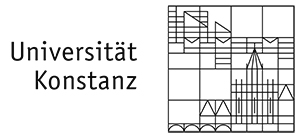
\includegraphics[width=0.15\textwidth]{./unisignet-klein}~\\[1cm]
\author{\\\\Author: \\
	Prakash Thapa
	\\\\\\  Supervisor: \\
	Prof. Dr. Marc H. Scholl \\ 
	Prof. Dr. Daniel Keim \\ 
	\\\\\\
	Christian Gr{\"u}en
	\\\\\\
	University of Konstanz
	}

	%Master Thesis in fulfillment of the requirements for the degree of
	%Master of Science (M.Sc.)
%\end{center}
%\end{titlepage}
\begin{document}
	%\definecolor{darkgray}{gray}{0.35}
\lstnewenvironment{fakeXML}[1][]{
\lstset{basicstyle=\footnotesize\sffamily,
linewidth=\linewidth,
breaklines=true, 
%numbers=left,
%stepnumber=1,
%numbersep=10pt,
frame=single,
framerule=1.0pt,
%backgroundcolor=\color{darkgray},
language=HTML,
identifierstyle=\color[rgb]{1,0,0},
emph={intersects}, emphstyle=\color{red},
keywordstyle=\color[rgb]{0,0,1},
commentstyle=\color[rgb]{0.133,0.545,0.133},
stringstyle=\color[rgb]{0.627,0.126,0.941},
morekeywords={xml, ref, xs, version, targetNamespace, minOccurs, maxOccurs}
}\lstset{#1}}{}

\lstnewenvironment{fakeJSON}[1][]{
	\lstset{
		basicstyle=\footnotesize\sffamily,
		keywords={typeof, new, true, false, catch, function, return, null, catch, switch, var, if, in, while, do, else, case, break},
		ndkeywords={class, export, boolean, throw, implements, import, this},
		sensitive=false,
		comment=[l]{//},
		morecomment=[s]{/*}{*/},
		morestring=[b]',
		morestring=[b]"
		linewidth=\linewidth,
		breaklines=true,
		escapeinside={\%*}{*)}
		numbers=left,
		stepnumber=1,
		numbersep=10pt,
		frame=single,
		framerule=1.0pt,
		language=JSON,
		emph={}
	}\lstset{#1}}{}

\colorlet{punct}{red!60!black}
\definecolor{delim}{RGB}{20,105,176}
\colorlet{numb}{magenta!60!black}

\lstdefinelanguage{json}{
	basicstyle=\normalfont\ttfamily,
	linewidth=\linewidth,
	numbers=left,
	numberstyle=\scriptsize,
	stepnumber=1,
	numbersep=8pt,
	showstringspaces=false,
	breaklines=true,
	frame=lines,
	literate=
	*{0}{{{\color{numb}0}}}{1}
	{1}{{{\color{numb}1}}}{1}
	{2}{{{\color{numb}2}}}{1}
	{3}{{{\color{numb}3}}}{1}
	{4}{{{\color{numb}4}}}{1}
	{5}{{{\color{numb}5}}}{1}
	{6}{{{\color{numb}6}}}{1}
	{7}{{{\color{numb}7}}}{1}
	{8}{{{\color{numb}8}}}{1}
	{9}{{{\color{numb}9}}}{1}
	{:}{{{\color{punct}{:}}}}{1}
	{,}{{{\color{punct}{,}}}}{1}
	{\{}{{{\color{delim}{\{}}}}{1}
	{\}}{{{\color{delim}{\}}}}}{1}
	{[}{{{\color{delim}{[}}}}{1}
	{]}{{{\color{delim}{]}}}}{1},
}
\lstdefinelanguage{sJSON}{
	keywords={typeof, new, true, false, catch, function, return, null, catch, switch, var, if, in, while, do, else, case, break},
	ndkeywords={class, export, boolean, throw, implements, import, this},
	sensitive=false,
	comment=[l]{//},
	morecomment=[s]{/*}{*/},
	morestring=[b]',
	morestring=[b]"
}

	\renewcommand{\lstlistingname}{Code}
	\maketitle
	\thispagestyle{empty}
	\newpage
	\section*{Abstract}
		%XML and NoSQL database are are two growing field in second generation database system, They share some similarities as well as they have some significant difference. 
This thesis focus on the  comparative analysis of these two database system. Based on the Use cases and existing solution, we will discuss the data processing, query pattern and  data retrial from these

		As dynamic data is growing rapidly, database vendors search for the alternative of classical database management system such as RDBMS. XML and NoSQL databases are two non-relational database management system growing since the popularity of Big Data. This thesis focus on the comparative analysis of these two new database system based on use cases and existing solutions. On the first part, our focus will be data migration from one system to another. We will also discuss  the performance of both systems based on standard queries.
		
		............
		...........
		............
	
	%\newpage
	\section*{Zusammenfassung(German Abstract)}
	XML und NoSQL


	%\newpage
	\section*{Acknowledgments}
	First of all I would like to thank Prof. Marc H. Scholl and Prof. Daniel A. Keim for being referee of this thesis. 

I am specially thankful to Dr. Christian Gr\"{u}n for being my advisor, and the valuable guidelines without which I could not move a step forward.

I would like to remember some of my colleague Klaus Herberth,  Nikhilesh Patil, Kritika Rajbhandari and Kiran Thapaliya for their support.  Also I would like to thank whole BaseX team. 
	\thispagestyle{empty}
	\newpage
	\tableofcontents
	\thispagestyle{empty}
	\newpage
	\section{Introduction}
	\setcounter{page}{1}
	\subsection{Motivation}
		\label{motivation}
			As the digital world growing very fast, the massive amount of data collected today in the field varying from business to scientific research, is becoming complex for storage, querying and providing mechanism for failover.  As the data collection grows so largely, the traditional data management tools e.g. relational database management systems(RDBMS) are struggling to handle such data effectively. The pre-design rigid schema structure of RDBMS made more complex for variety of data.  High data velocity where massive read and write operations possible from different geographic locations, storage of structured, semi-structured and unstructured data in gigantic volume, together is refer as  \textit{Big Data}. This has become a global phenomena which added more complexities on RDMS.
			
			New database technologies  NoSQL and  XML Databases came into existence to overcome above mentioned problems of RDBMS. These systems are not just able to solve the issues of existing systems, but also rise as alternative in their way. Both these new technologies focus on varieties of data in large volume, dynamic schema and scalability.
			%introduction to problem
			
			There are some research analysis between NoSQL and RDBMS. \cite{nance2013nosql} examine the pro and cons of both NoSQL and RDBMS, \cite{cattell2011scalable} analyze similarities between scalable SQL and NoSQL databases, \cite{hadjigeorgiou2013rdbms}  compare the performance between MySQL cluster as RDBMS and Mongodb as NoSQL Database.  There are also some research related to RDBMS with XML or XML Database(~\citet{jiang2002xparent}, \citet{shanmugasundaram1999relational}). But there are not much more research in the field of NoSQL and XML database together. So this thesis focus on these two new database systems. Migration of Data from XML database to NoSQL as well as performance of both system based on standard query will be examined.
			......
			....
	
	\subsection{Contribution}
		%\input{includes/1/contribution}
		The main contribution of this thesis is that it provides the necessary techniques and algorithms for migrating data from an XML database to NoSQL databases.  More specifically, it will focus on databases like MongoDB, Couchbase and Rethinkdb as NoSQL databases and BaseX as XML Database. To approach this challenge, it is first necessary to understand the general architecture and data model of each of these databases as well as the way how they are queried.The performance comparison of these two systems will be based XMARK dataset and its 20 standard queries~\citep{xmark/original}. These 20 queries of XMARK project will be translated to each of NoSQL databases.
		
	\subsection{Scope of Thesis}
	%The translation process use in this thesis from One format to another is based on XMark Dataset.
	.....
	....
	\subsection{Overview}
		This thesis is divided into three main sections. Section~\ref{nosql-xml-database}, we will discuss the two new databases system and the scope of thesis. Section~\ref{semi-structure-data} defines the techniques and necessary algorithms to convert XML  to JSON. In Section~\ref{sec:four}, focuses on the performance tests and comparative analysis of each of the NoSQL databases with BaseX, based on the XMark benchmarking project.		
			
	\label{nosql-xml-database}
	\section{NoSQL and XML Databases}
	\subsection{XML Database}
	XML Database or sometime written also Native XML Databases(NXDs) are document oriented databases that store XML data and all component of XML data based on a specified model called XDM. XML document is the fundamental unit of storage, so each document should be in a valid XML format.
	XQuery 1.0 and XQuery 3.0 are standards query languages recommended by W3C for NXDs. XQuery also includes XPath as sub-language. In addition to XQuery and XPath, XML databases also support XSLT, a method of transferring XML to other documents like HTML, plain text and XSL Formatting Objects.
	\subsubsection{BaseX}
	BaseX is a Native XML database management system and XQuery Processor. It uses tabular representation of XML data tree to store XML document~\citep{www/basex}. In this dissertation, BaseX is represented as XML database.
	....
	\subsection{NoSQL Database}
	NoSQL database "Not Only SQL" is distributed data management system for large and variable data. The main focus of any NoSQL database are scalability, performance and availability~\citep{hecht2011nosql}.
	Based on the Data model and design architecture, NoSQL databases are categorized into 4 groups:
	\begin{itemize}
		\item \textbf{Key/Value store}
		The Data representation of key-value stores are based on attribute pair, the data model is expressed as collection of $<$$key$,$value$$>$ tuples. The key is unique and value can be variable. The query operation on data can be uniquely performed by a key. There are no alternative ways to access or modify data without key.  DynamoDB, Riak, Redis are some examples of key-value stores.
		\item \textbf{Document oriented databases} are based on semi-structured data model, where unique key store a value that contains a tree like structure called \textit{document}. It is enclosed with key-value pair in JSON or in JSON like data format~\citep{hecht2011nosql}. In document store database, data can be access by using key or specific value. Some of the examples of document store databases are Mongodb, Couchbase, RethinkDB, CouchDB etc.
		\item \textbf{Column family} is also known as wide-column database stores data tables as section of a column. Cassandra, BigTable, HBase are categories as wide column database.
		\item \textbf{Graph databases} are based on graph theory. In these databases, data is represented as graph that is in the form of nodes and edges similar to social network. They store entities and relationship between these entities. Neo4J and OrientDB are two example of these databases.
	\end{itemize}
	As there are many categories and varieties of database system, our focus in this thesis is limited to document oriented databases of NoSQL databases.
	\subsubsection{MongoDB}
	%MongoDB is schema-free database system that manage data in the concept of database, collection and documents. A database contains one or more collections(can be compare to tables of RDBMS) which stores documents. Collections may contain any type of documents but generally they have documents with  similar schema. Data has flexible schema where collections do not enforce document to structure rather requirements of the application. Documents are modeled as a data structure following the JSON format which actually store as BSON, a binary variant of JSON, supports additional data types like ObjectId, timestamp, datetime etc.
		MongoDB is a schema-less document-oriented database developed by MongoDB Inc. with the support of Open Source community. 
\subsubsection{Data design} 
\paragraph{Document}
	A document is abstract and storable unit in MongoDB. It is the data structure expressed in the form of JSON and is stored in BSON, a binary variant of JSON that supports additional data types like ObjectId, timestamp, datetime etc. All the accessible data including database records, query selectors, index specifications, server configurations etc. are represented as documents. An example  MongoDB document is given in Figure~\ref{sample-mongodb-document}.
Every document is referenced with a unique key. A document is retrieved either by the key or any other attribute of the document. Collection in MongoDB is a group of documents and it is stored in a database. It is more convenient to group similar structured documents in a collection but not mandatory. MongoDB has two principles that allow the users to represent the relationships between the documents: \textit{references} and \textit{embedded} documents~\citep{mongodb:org}. 
\begin{itemize}
\item {Embedded:}\label{mongo:embedded}
    In Embedded document, data is nested. The documents are structured as sub-document in the form of Arrays or Objects~\citep{nosql/comparision}. 
    \item{Reference:}
    Unlike RDBMS, MongoDB has no support for joins, therefore related data is stored in a single document. In some cases, the related data can be stored in a separate collection. The relationship between data can be created by including links and references from one document to another as shown in Figure~\ref{fig:mongodb-ref-doc}.  The references between the data can be created in two ways:
\begin{itemize}
	\item {\textbf{Manual references}}
		In manual references, the application handles the relationship between documents by referencing \textit{\_id} field of one document to other. 
	\item \textbf{Database reference}(\textit{DBRefs})
	In  DBRefs reference, a first document's primary index field, collection name and optional database name of a document is used to reference to another document.
\end{itemize}



	% 	A document can be refer to another document with the help of collections of references.  where as referencing both collection name and database, MongoDB allows a document reference to multiple database.   With the reference of collection, a document can be reference to another document belonging different collection.
\end{itemize}

\begin{figure}[h]
	\centering
	\subfloat[Reference document]{
		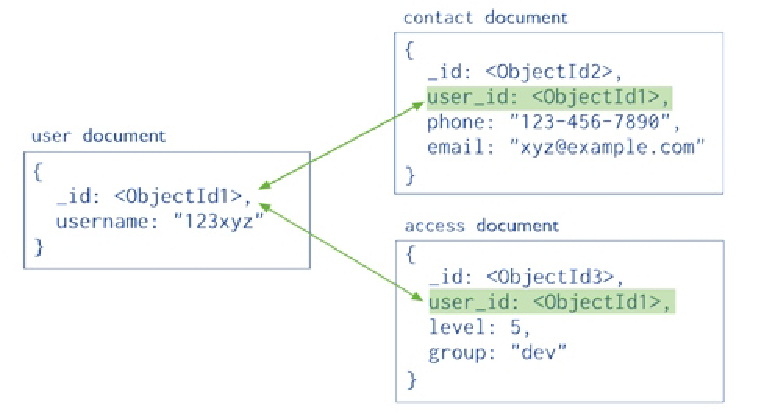
\includegraphics[width=.5\textwidth]{img/mongodb-reference}
		%{img/mongo/mongodb-reference}
		%\caption{R-tree structure}
		\label{fig:mongodb-ref-doc}
	}
	\centering
	\subfloat[Embedded document]{
		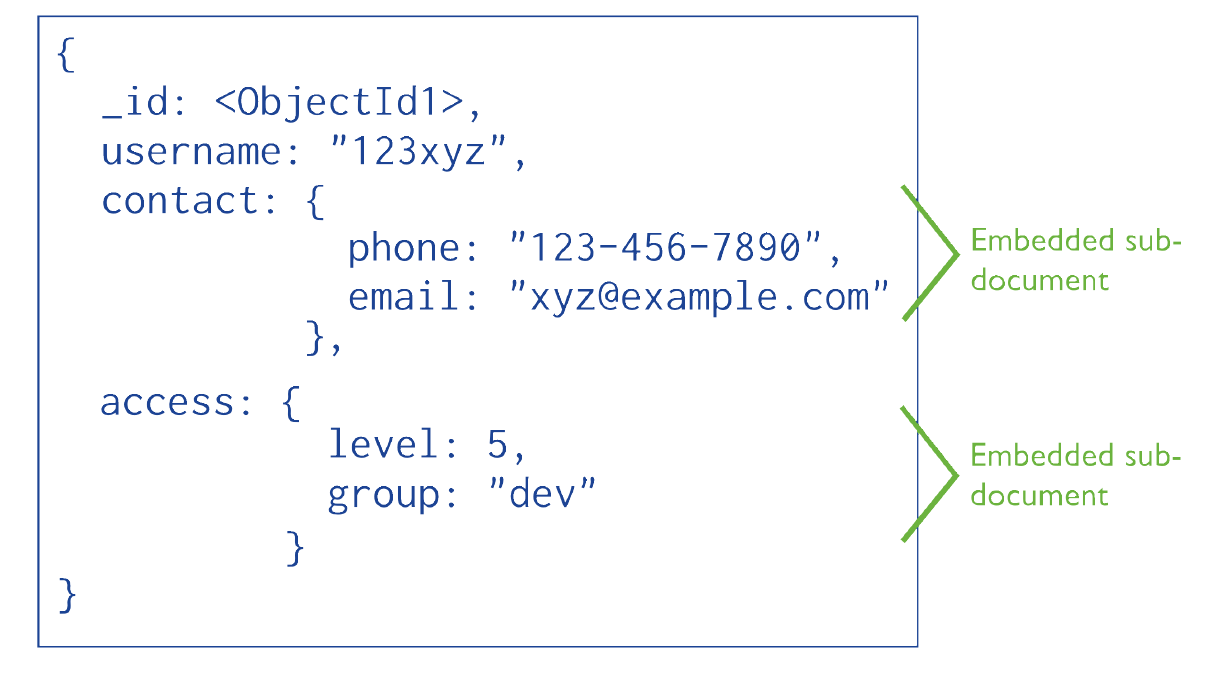
\includegraphics[width=.46\textwidth]{img/mongo/mongodb-embedded}
		%\caption{R-tree}
		\label{fig:mongodb-emb-doc}
	}
	\caption{MongoDB document structure~\citep{mongodb:org}}
	\label{fig:mongodb-doc}
	
\end{figure}

	\begin{figure}[h]
	\begin{lstlisting}[language=JSON,basicstyle=\scriptsize]
	{
		_id : "1"
		title : " MongoDB ",
		last_editor : "172.5.123.91" ,
		last_modified : new Date ("9/01/2015") ,
		body : " MongoDB is a..." ,
		categories : ["A", "B"] ,
		reviewed : false
	}
	\end{lstlisting} 
	\caption{MongoDB sample document}
	\label{sample-mongodb-document}
\end{figure}

\subsubsection{Indexing}\label{mong-xmark-indexing}

Each document in MongoDB is uniquely identified by a field \textit{\_id} which is also a primary index. Hence, the collection is sorted by \textit{\_id}~\citep{nosql/comparision}.
Apart from the primary index, MongoDB provides a mechanism to create secondary indexes for all fields of document. It supports various user defined indexes for field values including single field index, multikey index, multidimensional index, geo-spatial index, text index and hash index.
%Single field, multidimensional and multikey indexes are organized using B-tree, whereas geospatial index is implemented using quad trees.Once index is defined on a field,
\begin{itemize}
\item \textit{Single field index} only includes data from a single field of documents in a collection. 
\item \textit{Compound index} holds reference to the multiple fields within a collection's documents.
\item To index a field that contains an array value, MongoDB provides special indexing called \textit{Multikey index}.
\item \textit{Text index} helps efficient search of a string in documents.
\end{itemize}
\subsubsection{Query Model}\label{mongo-query-model}

%\todo{modify with christian's suggestions}
Queries in MongoDB are expressed in a JSON-like syntax and are sent to MongoDB as BSON objects by a database driver\citep{orend2010analysis}. A query can be specified by exact match on the embedded document or by using individual field with a \textit{dot notation}. It is used to access an element in document of an array or an object in the form of  $<$$array$.$index$$>$ or  $<$$object$.$childobject$$>$. For general queries, mongo shell can be used. It is an user friendly JavaScript shell that allows to implement callback functions to manipulate the data returned by the queries.  
\par
The Query model supports the following features:
\begin{enumerate}
	\item Queries over documents, embedded subdocuments and arrays
	\item Comparison operators
	\item Conditional Operators
	\item Logical Operators: AND and OR
	\item Sorting 
	\item Grouping
	\item Aggregation per query
\end{enumerate}

The \textit{find()} method is the most common way to retrieve data from a collection. It returns the subset of documents from specified collection with given criteria that are passed as parameters. If no any parameters is given, it returns everything from a collection.  The General syntax of find operation is given in Code~\ref{mongodb-find-sample}.
\begin{lstlisting}[language=JSON,caption=\textit{find} in MongoDB, label=mongodb-find-sample][H]
    db.collection.find(query, projection) 
\end{lstlisting}
 The \textit{query} specifies the criteria of document of a collection name \textit{collection}. The \textit{projection} selects of attributes of an documents to be return. For example, Code~\ref{mongodb-find-real} return the \textit{name} and \textit{age} from a collection  \textit{people} of country \textit{France} and \textit{age} is less than 5. 
\begin{lstlisting}[language=JSON,caption=\textit{find()} with query and project, label=mongodb-find-real][H]
    db.people.find({country:"France", age:{$lt:5}}, {_id:0, age:1, name:1}) 

\end{lstlisting}

\par
\paragraph{Aggregation Frameworks:}
 The \textit{find} method is not sufficient for the complex database queries like aggregation, grouping  and advanced data manipulation. MongoDB provides two frameworks for advanced query as well as parallel processing for the large collection:
 \begin{itemize}
		\item{ \textbf{Aggregation pipeline}} allows to execute series of operations using different operators like filtration, projection to produces desire result or performs aggregate operation.  It can be used for a single collection and uses  data operators like match, group, project, etc. in different stages. Every stage convert the documents as they pass through the pipeline. Data operators can be used  in any numbers of times.  The \textit{aggregate} function is responsible for this framework where it operates on a collection passing  entire documents into a pipeline. By using proper filtration operators like  skip, match and limit at the beginning  stage of the pipeline,  the frameworks can take advantages of existing indexes with processing scope limited to subset of documents, hence produces better performance in following stages~\cite{mongodbaggregation}. The aggregation pipeline has many limitations including data types, memory restriction to operators and output size~\cite{nosql/comparision}. Only 100 MB of RAM is assigned to pipeline stages. If this limit exceeds, the query will be broken. An option \textit{allowDiskUse} must be enable to write data to temporary files during staging.
		
				   \begin{lstlisting}[language=JSON,caption=An example Aggregation pipeline in MongoDB, label=mongodb-aggregation-pipeline, basicstyle = \scriptsize][h]
            db.open_auctions.aggregate([
                {$match:{reserve:{$exists:true}}},
		       {$project:{_id:0,reserve:{$multiply:["$reserve",2.20371]}}}
		       ]);
		  \end{lstlisting}
		  
		  \item{\textbf{MapReduce}} is a data processing framework design to support large volumes of data that goes beyond the limitations and restriction of aggregation pipeline.  In mapreduce,  \textit{map} function applies to each input document and emits the key-value pair as output. Any arbitrary sorting and limiting  of single collection is performed before map stage. The reduce applies to the map's output where a key is associated with multiple values to return the aggregated data. The output of \textit{reduce} may pass optionally through finalize function to further process the result. Mapreduce functions are written in JavaScript and executed in MongoDB's demon process ~\cite{mongodbaggregation}.  Unlike pipeline framework, Map-reduce support options for choosing to store result  data in a node as collection or return the output. Table~\ref{mongdb-mapreduce} illustrates a Mapreduce implementation in MongoDB. Two JavaScript function are defined for map and reduce. The \textit{runCommand} executes these functions in a collection.
		  
\end{itemize}		

\begin{longtable}{c|c}
\caption{Mapreduce in MongoDB}
 \label{mongdb-mapreduce}\\
	
	{\textit{map}} function(a) & {\textit{reduce}} function(b)\\
	\hline
	\begin{minipage}{.4\textwidth}
		\centering		
		\begin{lstlisting}[language=XML,basicstyle = \scriptsize,label=couchbase-map-sample]
map = function() {
           if(this.reserve){
            emit(this._id, this.reserve);
           }    
        };	
		\end{lstlisting}		
	\end{minipage} &
	\begin{minipage}{.49\textwidth}
		\centering
		\begin{lstlisting}[language=JSON, basicstyle =\scriptsize, label=couchbase-reduce-sample]
reduce = function(key,values) {
            return Array.sum(values);
        };
};
		\end{lstlisting}
	\end{minipage}
	\\
	\hline
	\multicolumn{2}{c}{
	    \scriptsize
	    
	Use: 	db.runCommand({"mapreduce" : 
	\textit{collectionName}, 
	                       "map" : \textit{map}, 
	                       "reduce" : \textit{reduce}})
		
	}
  	
  	\\
	\hline
	
\end{longtable}

%end here



\begin{comment}


\paragraph{System Architecture}
MongoDB can be run in two modes. In stand-alone mode, a single \textit{mongod} demon runs in a single node without any distribution and in shared mode various services are distributed to several nodes. 
\begin{figure}[h]
	\centering
	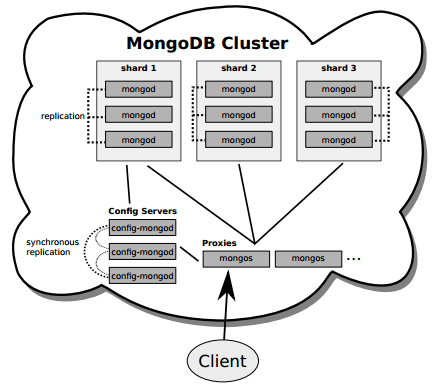
\includegraphics[width=0.5\textwidth]{img/mongo/clusters}
	%\caption{R-tree}
	\label{fig:mongodb-clusters}
\caption{MongoDB Clusters}
\end{figure} %reference




\end{comment}
	\subsubsection{Couchbase Server}
	%Couchbase Server is NoSQL database that can be used both as a key-value store as well as document store system. As key-value store, it is able to store  multiple data type such as strings, numbers, datetime, and booleans as well as arbitrary binary data. The key-value generally treated as opaque Binary Large Object(BLOB) and don't try to parse it. For document store, data need to be store in the valid JSON format. Data in Couhbase Server are stored in logical unit called Buckets. These buckets can be technically compare as \texttt{database} in Mongodb or other RDBMS. All data type other than JSON can be retrieve only by their key. So it is important to check meta type of data stored in a single document before retrieval. Unlike MongoDB, Couchbase server Don't have concept of collections, so category of documents are identified by user defined type or group.
		 Couchbase Server is designed to be an operational data store for real-time data access. It is a NoSQL database that serves both as key-value and  document-oriented database. As a key-value store, it is able to store any type of data including  strings, numbers and binary data and the data is generally treated as an opaque Binary Large Object(BLOB) that do not try to parse it at the time of query. when being used as document store, data is stored in a valid JSON format. The data in Couchbase is stored in logical unit called buckets. These buckets  are isolated to each other and have their own RAM quota and replica settings. Buckets can be compared with \texttt{database} in Mongodb or other RDBMS. Couchbase recommends few numbers of buckets in a single cluster. A Bucket contains any type of data but data other than JSON, it can be retrieved only by its key. Therefore, it is important to check meta type of data that is stored in a single document before fetching. Each document is stored independently and there is not the notion of grouping documents like collections in MongoDB or tables in other RDBMS. The documents is separated by a user-defined type to distinguish the such documents.  For example, all the documents that are in \textit{user} and \textit{post} collections of MongoDB can be represented in Couchbase by adding a new field \textit{documentType}  in each document  with value \textit{user} and \textit{post} respectively.  
\label{cb-metadata}
\paragraph{Metadata}
For every value stored in a bucket, Couchbase Server generates following meta information that is associated with a document~\cite[p. 26]{cb/ostrovsky2014pro}. 
\begin{itemize}
	\item{Expiration}
		The Time to Live(TTL) also named as expiration time is the life time of the document. The default value of TTL is 0 that indicates document will never expire and also can be set as Unix epoch time after which document is removed.
	
	\item{Check-and-Set(CAS)}
		The CAS value is 64-bit integer that is updated by server when associated item is modified. It enables to update information only if unique identifier matches the identifier of the document that needed to be updated. CAS is used to manage concurrency when multiple client attempts to update the same document simultaneously. 
	\item{Flags} are 32 bit integer and are set of SDK specific use. For example, format in which data is serialize or data type of the object being stored.
\end{itemize}	
In addition of TTL, CAS and flags, three other meta information are stored at the time of document creation. The document's key \textit{id} is saved as part of metadata, \textit{type} is the type of a document either \textit{json} or Base64 encoded string for all other.
\paragraph{\textit{Document key}}
Every value in Couchbase Server is saved in unique key called document key. Unlike MongoDB, Couchbase  do not generate document key automatically and 250 characters string should be manually generated.
%In case of XMark data each \texttt{id} attributes of  \texttt{item}, \texttt{person}, \texttt{open\_auction}, \texttt{category} represent as key. In case of  \texttt{closed\_auction} and  \texttt{edge} key can be manually generated. 
\begin{figure}[h]
	\centering
	\subfloat[Views in Document Design]{
		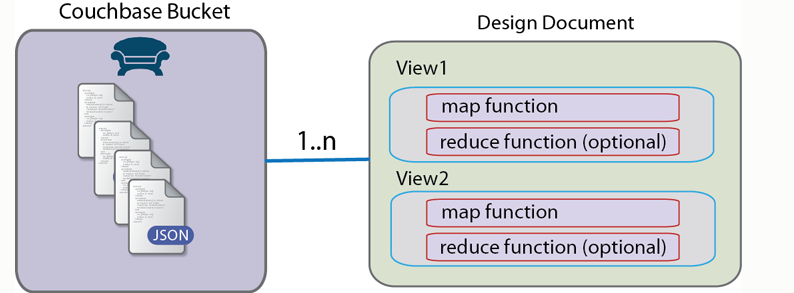
\includegraphics[width=0.4\textwidth]{img/cb/Small_view_elements}
		\label{fig:cb-views-design}
	}
	\centering
	\subfloat[View's Workflow]{
		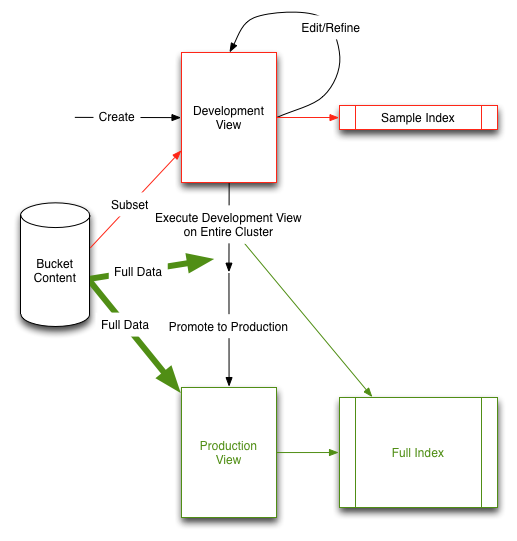
\includegraphics[width=0.4\textwidth]{img/cb/view-types-workflow}
		\label{fig:cb-views-workflow}
	}
	\caption{Couchbase Server's Document Design ~\citep{couchbasedocs}}
	\label{fig:cb-views-document-design}	
\end{figure}

\paragraph{Bucket and vBucket}
Couchbase Server uses data bucket as a logical container of information that provides a logical grouping of physical resources within a cluster~\citep{lichtenberg2013nosql}. Documents in Couchbase do not have their fixed schema and multiple documents  with different schema can be stored in same bucket. One or more attributes in documents are added to differentiate the various objects stored in a bucket and create indexes on them. Each bucket is split into 1024 logical partition called vBuckets. A vBucket is treated as a owner of subset of key where every key belongs to a vBucket~\ref{fig:cb-vbucket}.  
%%why we need vbucket

\begin{figure}[h]
	\centering
	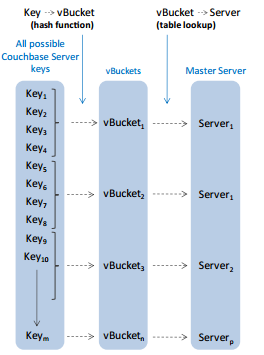
\includegraphics[width=0.4\textwidth]{img/vbucket2}
	\caption{ Couchbase  vBucket ~\cite{couchbasedocs}}
	\label{fig:cb-vbucket}
\end{figure}
%where is reference of images

\paragraph{Data Model}%repeat check once
A document is a basic unit of data manipulation in Couchbase  as a document store. All the documents are stored in JSON format without a predefined schema.

\paragraph{Querying and Indexing}
Query in Couchbase has to be done against pre-materialize views. The goal of view is to select the data, extract the attributes and information as client's need  and to produce the index on selected information. Views are defined in a specific kind of document called \textit{design document}~\ref{fig:cb-views-design}. These documents are bounded to a single bucket and cannot be executed from other bucket. The design document holds JavaScript code that implements \textit{Mapreduce} operations to create view's index in user defined format. The Mapreduce is achieved by two functions \textit{map} and reduce. Table~\ref{tbl:cb-mapreduce} illustrate a sample mapreduce function in Couchbase.

The \textit{map} function in design document identifies data from collection, process, filter them and output transformed values. Each document in a bucket is submitted to the \textit{map } function where document and metadata associated with the document are supplied as parameter to the \textit{map} function. After filtration, the \textit{emit} function in map returns the result as set of key/value pairs that are index. The output of map function can be zero or more "rows" according to the filter used in \textit{emit()} function. Each \textit{emit()} function returns a single row but can be called multiple times inside a single map function. The first parameter in \textit{emit} function is searchable text key and second parameter is the value.
The \textit{reduce} function is used to aggregate the numeric value generated in map phase. Couchbase has built-in reduce functions like \textit{\_count}, \textit{\_sum} and \textit{\_stats} aggregation. Table ~\ref{tbl:cb-mapreduce} illustrate an example of MapReduce  in Couchbase. The emit function at map phase returns the \textit{id} of document  as key and the price greater than 40 from documents that contains \textit{doctype} value "closed\_auctions". In \textit{reduce} phase, the the keys are grouped and values are counted.

%start here 
 In contrast to MongoDB,  Couchbase's queries are closely associated with client SDK where each operations has to perform through SDKs. On-demand query language  named "N1QL" is also in  progress of development but still stable version has to be released~\cite{couchbasen1ql}.


%end here from benchmarking sections.
\begin{table}[H]
\begin{longtable}{c|c}
	\caption{Mapreduce in Couchbase}
	\label{tbl:cb-mapreduce}\\
	\textit{map()} & \textit{reduce()}\\
	\hline
\begin{minipage}{.6\textwidth}
\begin{fakeJSON}[label=cb-mapreduce-map,basicstyle =\scriptsize]
function (doc, meta) {
   if(doc.doctype && doc.doctype=="closed_auctions"){
     if(doc.price){
       if(doc.price > 40) {
	      emit(doc.id,doc.price)
     	}
    }
  }
}

\end{fakeJSON}	
\end{minipage} &
\begin{minipage}{.2\textwidth}
\begin{fakeJSON}[label=cb-mapreduce-reduce]
	_count
\end{fakeJSON}
\end{minipage}\\
\end{longtable}
\end{table}


	
	\subsubsection{RethinkDB}
	%RethinkDB is distributed database system to store  JSON documents that uses efficient query languages named ReQL which automatically parallelize queries in multiple machines. RethinkDB has similar concept of store database like MongoDB. A database contains schema-less table, where documents are stored in the form of JSON. Unlike MongoDB, RethinkDB query language supports join queries between tables.
		RethinkDB is an open-source distributed document-oriented database system to store JSON documents. One of the unique feature of RethinkDB is the changefeed by the server to the client. 
Instead of a client request, the changes in database is streamed to the client application in realtime. In case of multi-users environment, any database  update is automatically notified.
\par
ReQL is the query language  of RethinkDB and it is based on three main principles:
 \begin{itemize}
 \item  It is  embedded  as programming language. Queries are constructed by making function call. 
 \item ReQL queries are chainable that can be passed as pipeline from one stage to another. Complex operation can be performed using series of simple queries together by using dot operators (\.) . 
 \item All the queries are executed in server without any intermediate network round trip between the server and clients.
 \end{itemize}
  
\subsubsection{Data Model}
There are two ways to model relationships between the documents: 
\begin{itemize}
	\item \textbf{Embedded arrays:} In this method, the related sub-documents are inserted with a specific key inside a document as in MongoDB ~\ref{mongo:embedded}. The advantages of using embedded arrays are:
		\begin{itemize}
			\item The Queries tend to be simpler. 
			\item If a dataset  does not fit into RAM, then the data is loaded  from the disk and it is faster compared to tables. 
		\end{itemize}
		Disadvantages of embedded arrays are: 
		\begin{itemize}
			\item Before any operation, data should be loaded into memory. In case of any updates, the document will rewrite the full array to the disk.
		\end{itemize}
		
	\item 
	\textbf{Multiple Table Approach:} In this approach, documents with similar structures are stored in multiple tables similar to collection in MongoDB. These tables are connected by reference key. Unlike embedded arrays, operation of a table does not required to load data from reference table in memory.
\end{itemize}

\subsubsection{Query Model}
RethinkDB's query language ReQL is embedded as programming language and JavaScript expressions can be used anywhere as a part of the query. The anonymous function, also known as lamda function, is a part of the query language that gives more flexibility for retrieving data. All the ReQL queries are chainable therefore, the dot \{.\} operator at any point of query can be extended to multiple levels as shown in Code~\ref{reql-chainable}.
	\begin{lstlisting}[language=JSON,caption=Chainable Query in ReQL, label=reql-chainable, xleftmargin=-40pt, 	basicstyle=\ttfamily\footnotesize][h]
		r.table("users").run(conn)
		r.table("users").pluck("last_name").run(conn)
		r.table("users").pluck("last_name").distinct().run(conn)
		r.table("users").pluck("last_name").distinct().count().run(conn)
	\end{lstlisting} 
The queries are built up on client side and send to the server when the \textit{run()} is called. Then the server automatically parallelized the queries into different nodes. whenever possible, the query execution is splitted into different cluster and data-centers.
\par
Unlike other NoSQL databases, RethinkDB supports join queries between the tables in one-to-many or many-to-many relationships in distributed manner. 
%start here from bechmarking section
%there should be some changes
\subsubsection{Indexing}
	RethinkDB uses B-trees to store indexes. When tables are created, there is an option to specify the attribute as a primary key. \textit{id} behaves as a primary key if the attribute is not specified and it is used to index the document. If there is no  primary key, a random unique string is automatically generated to index the document. Beside the primary index, RethinkDB supports simple, compound, secondary, geospatial indexes. Beside that any arbitrary expression can be used to create index from any type of user defined expressions like lamda functions. Every query including update operations uses only one index.
	 Only \textit{getAll()} \textit{between()}, \textit{eqJoin()} and \textit{orderBy} functions can use secondary index.		
	%\subsection{Summary}
	\paragraph{}
	%All document oriented NoSQL database store data in the form of JSON or JSON like format and XML is the basic unit of storage for XML database. for data migration, it is necessary to understand the properties of XML and JSON Data format.	
	
\label{semi-structure-data}
\section{Semi-structured Data: XML and JSON}
		XML, by definition a textual markup language where data elements are ordered by nature: \textit{string} is core data type from which richer data types e.g. integers, floats and user-defined abstract data types are derived~\citep{xmark/original}.
		A JSON or JavaScript Object Notation is programming language model. It is minimal textual and a subset of JavaScript. JSON document consists of two data structures:
		\begin{itemize}
			\item Objects, an unordered collection of name-value pair that are encapsulated by curly braces \{ and \}. The key is a string encapsulated in double quotes and must followed by a column(:) to it's value. The key must be unique for each object.
			%TODO:   which are numbers of key value pairs
			\item Arrays, which are an ordered list of values
		\end{itemize}
		A JSON value can be Object, Array, number, string, \texttt{true}, \texttt{false} and \texttt{null}.
		%JSON documents consists of a number of key-value pair (also called attribute-value pair)
		\subsection{Problem to translate from XML to JSON}
		JSON and XML look conceptually similar as they both text based markup language, which are designed to represent data in human-readable form, exchangeable across multiple platforms and parseable by common programming language. When we look at them first, they appear to be quite similar, with difference only in their syntax. But it turns out that they are fundamentally incompatible, as we will see in the following~\citep{lee2011jxon}.
		
		\paragraph{Root node}
		Each XML document have a document node. In contrast, the JSON does not have one. In practice, XML node is implicitly created in the model and does not have a textual representation.
		\paragraph{Anonymous values}
		JSON support the anonymous values(also refer as string value). They only acquire names by being referenced in an object. for example \ref{tbl:Anonymous-xmljson} is valid JSON. An XML valid document should have a root element followed by  non-mandatory child text or attributes.
		
\begin{longtable}{c|c}
	\caption{Anonymous values of JSON in XML}
	\label{tbl:Anonymous-xmljson}\\
	\textbf{JSON} & \textbf{XML}\\
	\hline
\begin{minipage}{.4\textwidth}
\begin{fakeJSON}[label=json-anonymous]
	["Hello World"]
\end{fakeJSON}	
\end{minipage} &
\begin{minipage}{.55\textwidth}
\begin{fakeXML}[label=xml-anonymous]
	<root>Hello World</root>
\end{fakeXML}
or
\begin{fakeXML}
	<root value="Hello World">
\end{fakeXML}
\end{minipage}\\
\end{longtable}
	
		\paragraph{Arrays}
		Arrays are native data types of JSON which does not exists in XML. There is no direct markup for array of Object from JSON to XML.
		\paragraph{Identifiers}
		XML is much more restrictive for identifiers as compare to JSON which allows any string to be an identifier. Translating from XML to JSON do not cause problem but in reverse case might lead to invalid XML. For example "Hello World" is a valid identifier in JSON but not valid attribute or element in XML as there exists a whitespace between two words.
		\paragraph{Attributes}
		JSON does not have the concept or representation for XML's attributes. When mapping from XML to JSON, attributes are translated to name object member along with other child elements. This information will be loss when mapping from JSON to XML.
		\paragraph{Namespaces}
		XML supports the concept of namespaces to provide uniqueness in element and attributes in XML document. Namespaces do not exists in JSON. Mapping QNames in XML with namespaces to JSON can lead ambiguous and duplicate names.
		\paragraph{Others}
		%TODO: {Processing Instructions, Character Set, Comments, Encodings}
		There are also some problem like processing instructions and  comments which XML supports but not JSON. Other issues for example character set and encoding are not easily exchangeable.
		
	\subsection{Mapping}
	XML and JSON have different data types. Compare to JSON, XML has more flexible data types. In Table~\ref{tbl:xml-json:types} is given types of data for simple XML and relevant JSON type.
	\lstset{
  frame=none,
  numbers=none
}
\begin{longtable}{c|c}
\caption{Translation of simple XML data types into JSON}
\label{tbl:xml-json:types}\\

\textbf{XML type definition} & \textbf{JSON type definition}\\
\hline

\begin{minipage}{.4\textwidth}
  \begin{lstlisting}
xs:string
  \end{lstlisting}
\end{minipage} &
\begin{minipage}{.55\textwidth}
\begin{lstlisting}
{
  "type": "string"
}
\end{lstlisting}
\end{minipage}\\

\hline
\begin{minipage}{.4\textwidth}
  \begin{lstlisting}
xs:boolean
  \end{lstlisting}
\end{minipage} &
\begin{minipage}{.55\textwidth}
\begin{lstlisting}
{
  "type": "boolean"
}
\end{lstlisting}
\end{minipage}\\

\hline
\begin{minipage}{.4\textwidth}
  \begin{lstlisting}
xs:float
xs:double
xs:decimal
xs:integer
(All Other Numbers)
  \end{lstlisting}
\end{minipage} &
\begin{minipage}{.55\textwidth}
\begin{lstlisting}
{
  "type": "number"
}
\end{lstlisting}
\end{minipage}\\
\hline

\begin{minipage}{.4\textwidth}
	\begin{lstlisting}
	(Remaining all others)
	\end{lstlisting}
\end{minipage} &
\begin{minipage}{.55\textwidth}
\begin{lstlisting}
{
	"type": "string"
}
\end{lstlisting}
\end{minipage}\\
\end{longtable}
For complex XML data type, there are two options in JSON, either object or array based on XML object.

\subsection{Migration from XML to JSON}
It takes different stages to convert XML data to JSON.
		\begin{enumerate}[label=Step\arabic*.]
			\item
			XML to JSON friendly XML: Convert standard XML data to JSON friendly XML.
			\item
			Data type of XML to JSON type: Define the data type of XML element whether it is array type or Object type or other scaler type.
			\item
			Final steps: Map XML to JSON object.
		\end{enumerate}
		\paragraph{Step 1}
		At first, all attributes of XML document are represented as ordered(first) child element of parent then attributes are deleted. There can more than one attributes which are inserted in order. XML node can contain both text node and element node as child, but JSON can have only key value pair. so each of text node which also  has element node as siblings moved to "childtext"(name of the element) node. At the end of first step, if an element has another element as child node, then it is represented as Object type of JSON. It is necessary to identify if a siblings of an element node(S) has same element name or not. If this condition exists, S is represented as the array in JSON. All the child nodes of all siblings are moved inside S node. If S is already  object type  then it is replace with array type  else new array is added. %In this algorithm, the loop of one action affect other, so they are looped independently.
		
		
		\begin{algorithm}[h]
			\DontPrintSemicolon
        	\begin{algorithmic}
        	\STATE Initialize $D = "{XML} document"$;
        	  	\FORALL{descendant-or-self node of  $D$,  $X$ which has attributes $A$  }
        			\STATE move  all attributes  $A$ to ordered child element of $X$\;
        		\ENDFOR
        		
        		\FORALL{descendant-or-self node of  $D$,$X$ }
        			\IF{ $X$ contains Text node and element node Both}
        				\STATE create new element "childtext" \;
        				\STATE move text node to "childtext" element \;
        			\ENDIF
        		\ENDFOR
        		
        		\FORALL{descendant node of  $D$,$X$ }
        			\FORALL{child element $C$ in $X$}
        				\IF{ $C$ has siblings $S$ with same \textit{name} }
        					\STATE convert $C$ as Array type\;
        					\STATE move child of $S$ into $C$ as $<$\_$>$ element\;
        				\ENDIF
        				\IF{ $C$ has child element }
        					\STATE convert $C$ as Object type\;
        				\ENDIF
        			\ENDFOR
        		\ENDFOR
        	\end{algorithmic}
        	\caption{Pseudocode to convert normal  XML to JSON friendly XML}\label{algorithm-JSONXML}
        \end{algorithm}
	
 \begin{algorithm}[h]
			\DontPrintSemicolon
        	\begin{algorithmic}
        	\STATE Initialize $D = "{XML} document"$;
        	  	\FORALL{descendant-or-self node of  $D$ as $C$}
        			\IF{ $C$ has no attribute "type" }
        				\STATE get content of $C$ \;
                        \STATE identify content type according to Table ~\ref{tbl:xml-json:types}. and add attribute to $C$ "type" \;
        			\ENDIF
        		\ENDFOR
        	\end{algorithmic}
        	\caption{ convert data type of XML to JSON data type(Step 2)}\label{algorithm-JSONXML-type}
        \end{algorithm}

\begin{longtable}{c|c}
	\caption{XML to JSON friendly XML(STEP 1)}
	\label{tbl:xmljson}\\
	\textbf{XML} & \textbf{ Algorithm~\ref{algorithm-JSONXML} }\\
	\hline
\begin{minipage}{.4\textwidth}
\begin{fakeXML}
<info>
  <name>
    <f>a</f>
  </name>
  <age>24</age>
  <ismarried>false</ismarried>
  <city name="Armonk"/>
  <state>NY</state>
  <contact>
	 home
    <p>993-330</p>
    <p>993-331</p>
  </contact>
</info>
\end{fakeXML}	
\end{minipage} &
\begin{minipage}{.55\textwidth}
\begin{fakeXML}
<info type="object">
  <name type="object">
    <f>a</f>
  </name>
  <age>24</age>
  <ismarried>false</ismarried>
  <city type="object">
    <name>Armonk</name>
  </city>
  <state>NY</state>
  <contact type="object">
	<childtext>home</childtext>
    <p  type="array" >
	   <_>993330</_>
	   <_>993-331</_>
    </p>
  </contact>
</info>
\end{fakeXML}
\end{minipage}\\
\end{longtable}

\begin{longtable}{c|c}
	\caption{XML to JSON friendly XML(STEP 2)}
	\label{tbl:xmljson-2}\\
	\textbf{Algorithm~\ref{algorithm-JSONXML}} & \textbf{ Algorithm~\ref{algorithm-JSONXML-type} }\\
	\hline
\begin{minipage}{.4\textwidth}
\begin{fakeXML}
<info type="object">
  <name type="object">
    <f>a</f>
  </name>
  <age>24</age>
  <ismarried>false</ismarried>
  <city type="object">
    <name>Armonk</name>
  </city>
  <state>NY</state>
  <contact type="object">
	 <childtext>home</childtext>
    <p  type="array" >
	   <_>993330</_>
	   <_>993-331</_>
    </p>
  </contact>
</info>
\end{fakeXML}	
\end{minipage} &
\begin{minipage}{.55\textwidth}
\begin{fakeXML}
<info type="object">
  <name type="object">
    <f type="string">a</f>
  </name>
  <age type="number">24</age>
  <ismarried type="boolean">false</ismarried>
  <city type="object">
    <name type="string">Armonk</name>
  </city>
  <state>NY</state>
  <contact type="object">
	 <childtext type="string">home</childtext>
    <p  type="array" >
	   <_ type="number">993330</_>
	   <_ type="string">993-331</_>
    </p>
  </contact>
</info>
\end{fakeXML}
\end{minipage}\\
\end{longtable}

\paragraph{Step 3}
	After Step 1. and 2., a complete JSON friendly XML is generated. All XML object and array are mapped to $<$$key$, $value$$>$ pair of JSON and their respective data types.
	\begin{longtable}{c|c}
	\caption{XML to JSON (STEP 3.)}
	\label{tbl:xmljson-convert-3}\\
	\textbf{XML(After step 2)} & \textbf{JSON}\\
	\hline
\begin{minipage}{.55\textwidth}
\begin{fakeXML}
<info type="object">
  <name type="object">
    <f type="string">a</f>
  </name>
  <age type="number">24</age>
  <ismarried type="boolean">false</ismarried>
  <city type="object">
    <name type="string">Armonk</name>
  </city>
  <state type="string">NY</state>
  <contact type="object">
	<childtext type="string">home</childtext>
    <p  type="array" >
	   <_ type="number">993330</_>
	   <_ type="string">993-331</_>
    </p>
  </contact>
</info>
\end{fakeXML}	
\end{minipage} &
\begin{minipage}{.5\textwidth}
\begin{fakeJSON}
{
    "info":{
      "name":{
        "f":"a"
      },
      "age":24,
      "ismarried":false,
      "city":{
        "name":"Armonk"
      },
      "state":"NY",
      "contact":{
	   "childtext":"home",
        "p":[
          993330,
          "993-331"
        ]
      }
    }
}
\end{fakeJSON}
\end{minipage}\\
\end{longtable}

%new section
\newpage
	
	%this section have to move to in conclusion and future work
	%\section{Related work}
	\newpage
	\section{Performance/Experiments}
	\label{sec:four}
		\subsection{XMark}
		\label{xmark}
			The XML benchmarking project XMARK~\citep{xmark/original} is one of the most popular and commonly used XML benchmarking projects to date. It provides a small executable tool called \textit{xmlgen} that can be used to create a synthetic XML dataset based on a fixed schema describing an Internet auctions database. xmlgen can be used to build a single record with a large, hierarchical XML tree structure. A factor is specified to scale the generated data, ranging from a few kilobytes to an arbitrary size, limited by the capacity of the system. The textual part of the resulting XML document is constructed from 17,000 most frequently occurring words of Shakespeare's plays.

\subsection{Dataset}\label{xmark-dataset}
The main entities of XMark data are in two groups. The first group consists of  \textit{person}, \textit{open\_auction}, \textit{closed\_auction}, \textit{item} and \textit{category}. The second group's entities \textit{annotation} and \textit{description} are natural language text and document-centric element structure. The relationship between the entities in the first group are expressed as reference and the second group entities are embedded into subtree of first group entities. Figure~\ref{fig:xmark-tree} shows the XMark dataset with the following properties:
\label{xmark:desc:each}
\begin{itemize}	
	\item
	\textit{people} is a collection of \textit{person} element that is connected to buyer and seller of \textit{open\_auctions}, \textit{closed\_auctions}, etc. Each person has an unique identifier \textit{id} to reference to another entities like open\_auctions and closed\_auctions.
	\item
	\textit{regions} is a collection world regions \textit{africa}, \textit{asia}, \textit{australia}, \textit{europe}, \textit{namerica} and \textit{samerica}. Each of these region has \textit{item} elements which are the objects for sale or already sold. Each \textit{item} carries a unique identifier \textit{id} and has properties like name, payment information, description and a reference to the seller that are encoded as elements. 
	\item
		\textit{open\_auctions} refers to current auctions that contains bid history(increase/decrease over time) with references to bidders and sellers, current bid, the time interval of bid accepted, the status of the transaction, a reference to the item being sold etc.
	\item
		\textit{closed\_auctions} contains auctions that are successfully completed. They have properties like buyer and seller information reference to \textit{person}, a reference to sold items, amount of price, quantity of sold items, date of transaction, type of transaction, and much more.
	\item 
		\textit{categories} is used to classify the items. Each category has a unique identifier used to reference an item, a name and a description.
	\item
		  A \textit{catgraph} links categories into a network.  The full semantics of the XMark dataset can be found in~\cite{xmark/original}.
\end{itemize}
The full ER-Diagram of XMark dataset is illustrated in Fig.~\ref{fig:xmark-schema}. 
\begin{figure}[H]
	\centering
	\subfloat[Reference in \textit{XMark}]{
		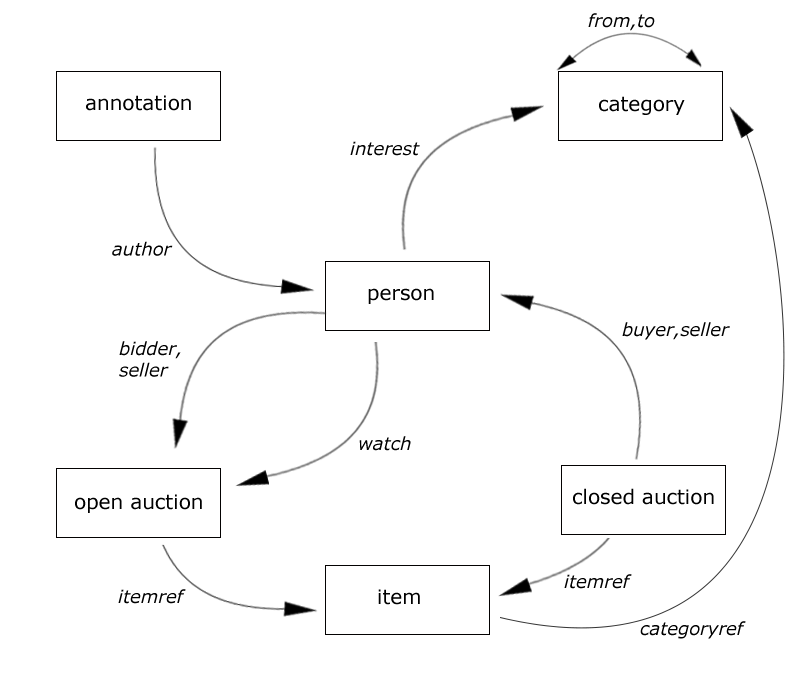
\includegraphics[width=0.40\textwidth]{img/xmark/101}{ %xmark-references.png
			\label{fig:xmark-reference}
		}
	}
	\centering
	\subfloat[Reference in \textit{XMark} dataset tree]{
		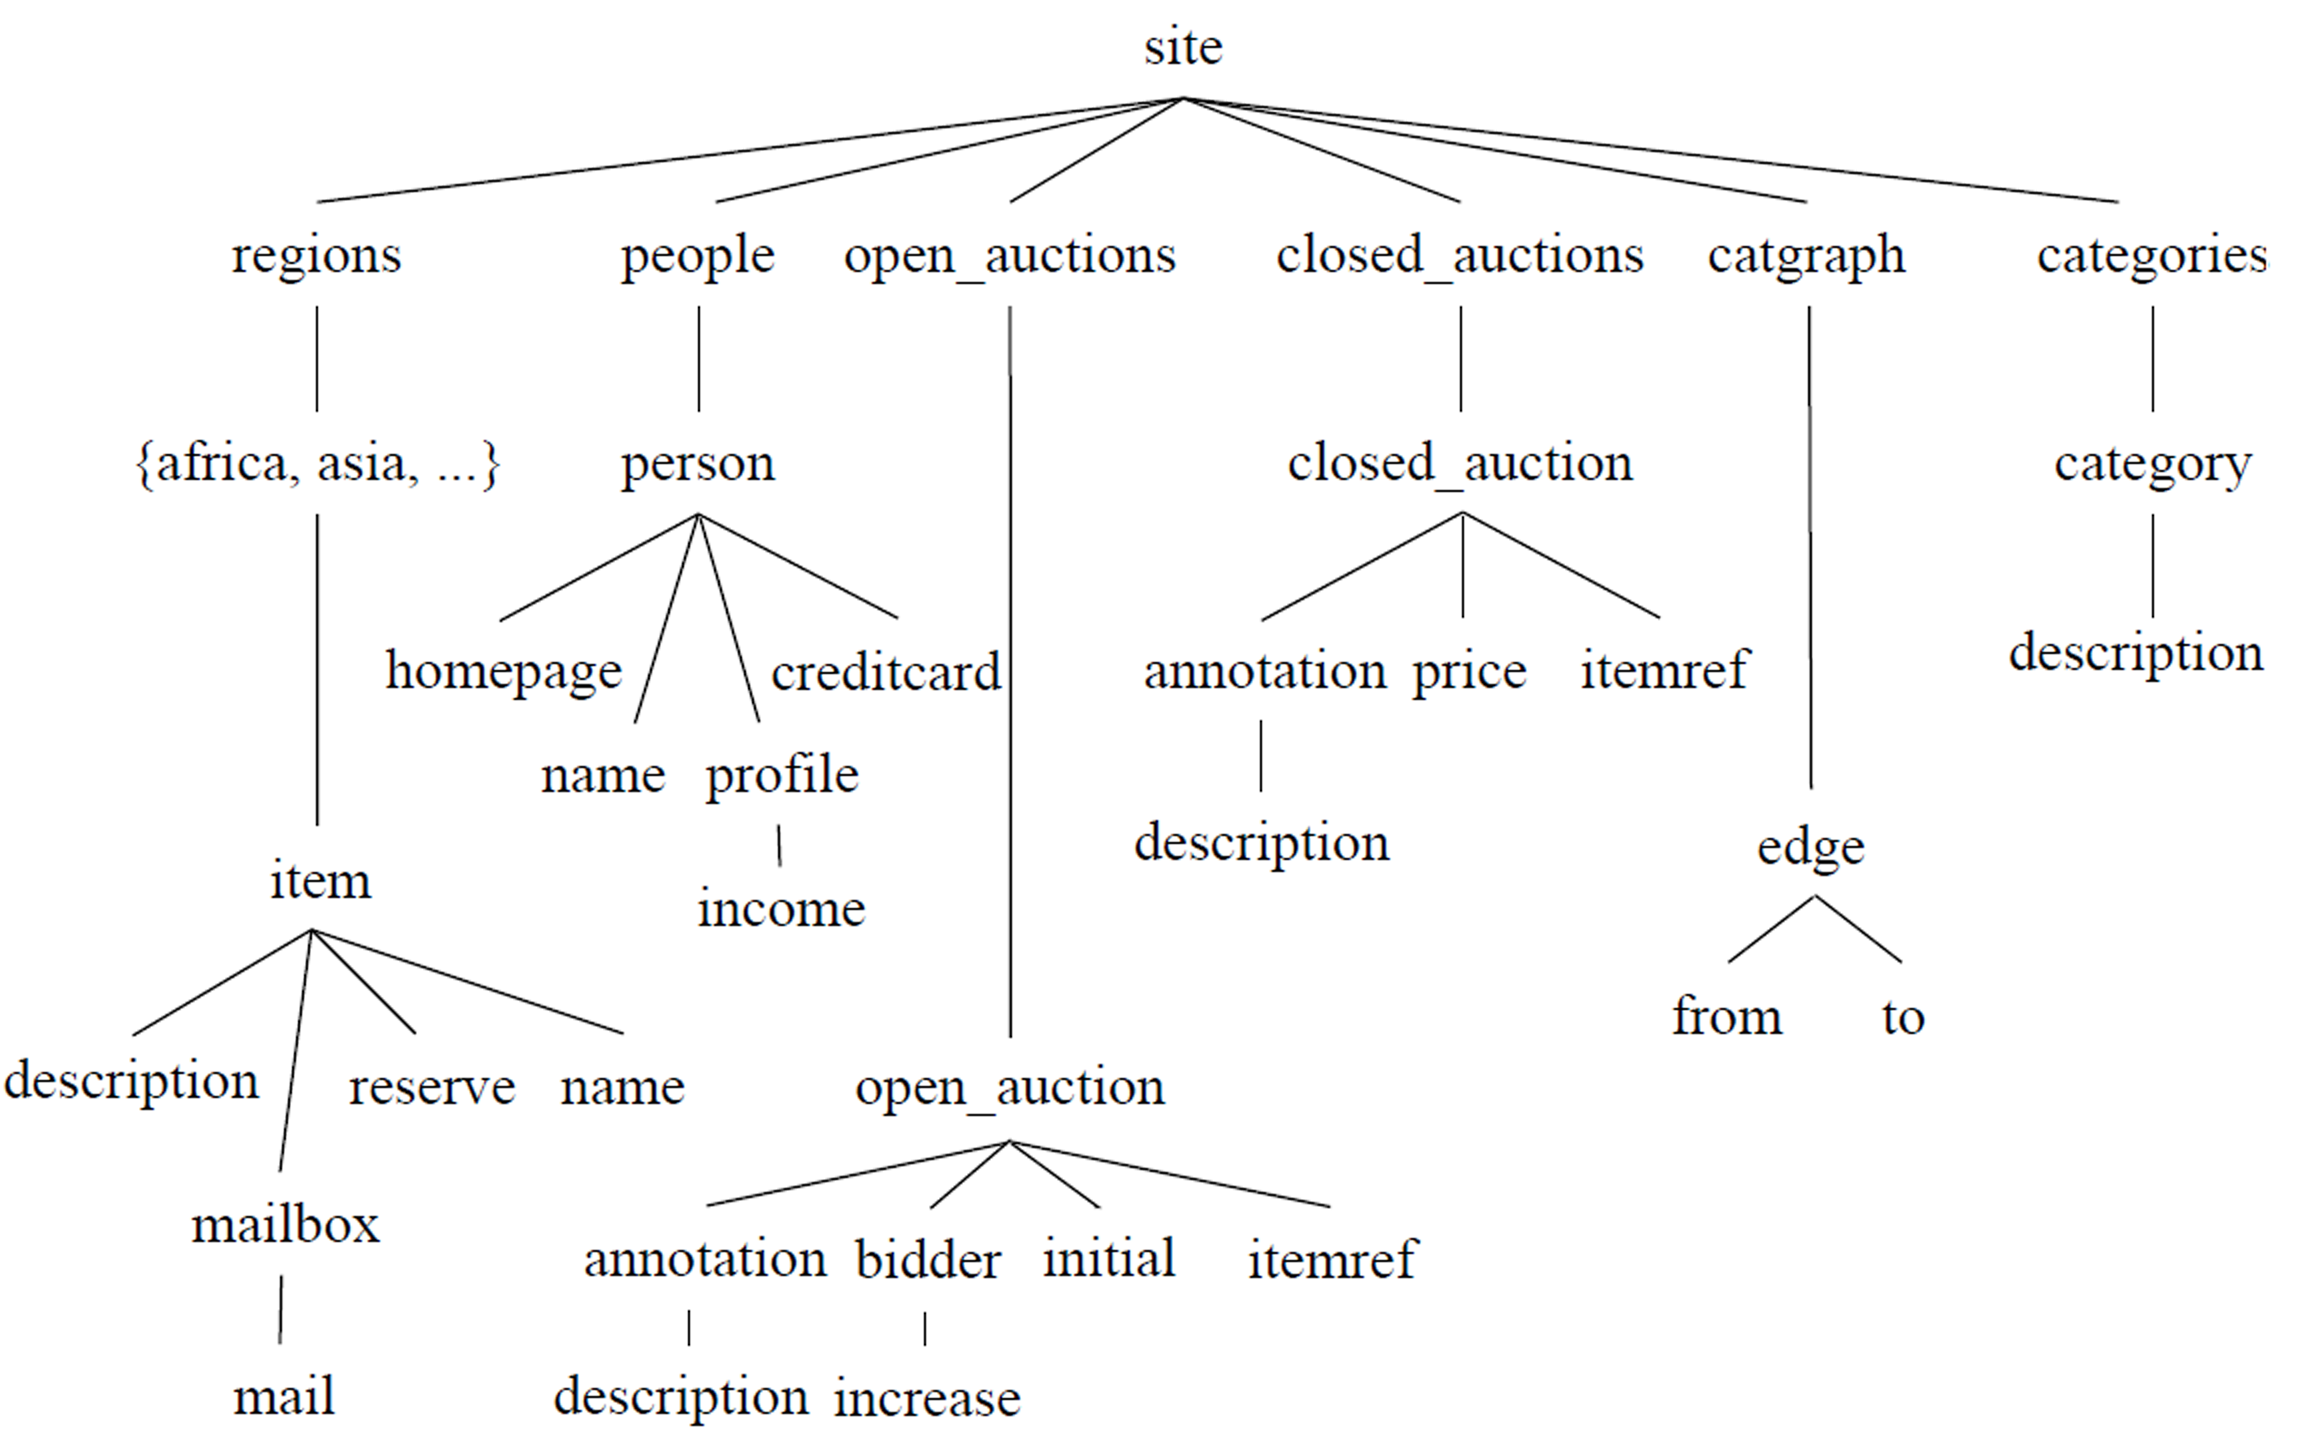
\includegraphics[width=0.4\textwidth]{img/xmark-tree.png}{
			\label{fig:xmark-tree}
		}
	}
	\caption{XMark data tree and reference~\citep{xmark/original}}
	\label{fig:xmark-tree-reference}
\end{figure}
\begin{figure}[H]
	\centering
	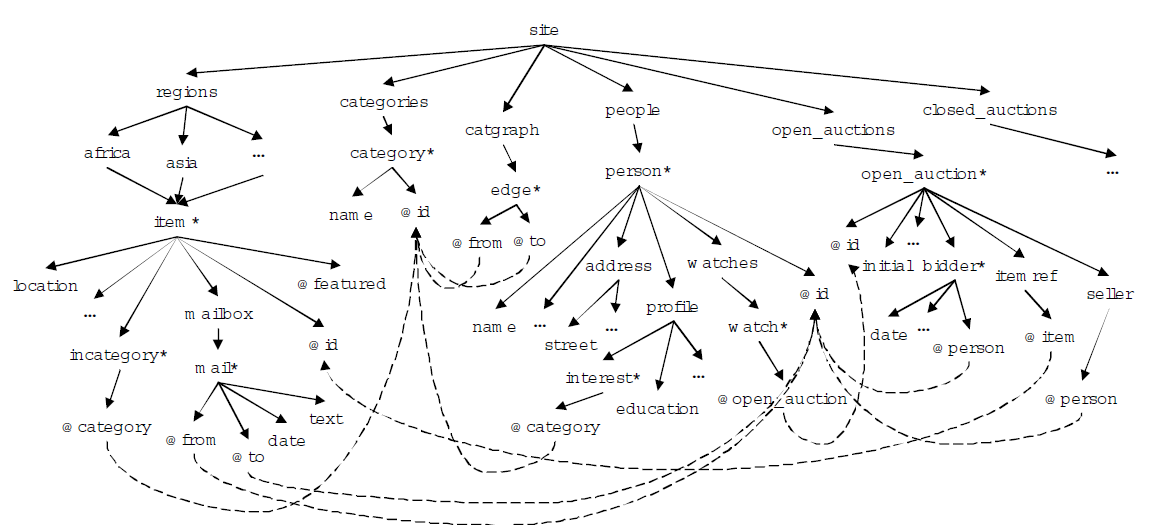
\includegraphics[width=0.90\textwidth]{img/xmark-schema-4}
	\caption{XMark ER-Diagram. Nodes, solid arrows, and dashed arrows represent schema elements (or attributes, with prefix '@'), structural links, and value links, respectively. Elements with suffix '*' are of SetOf type\citep{xmark/schema-sumerize}}
	\label{fig:xmark-schema}
\end{figure}

\subsection{XMark Queries}\label{xmark-queries}
The XMark project contains XQuery queries that focuses on the various aspect of language such as aggregation, reference, ordering, wildcard expressions, joins, user defined functions, etc.\citep{xmark/mlynkova2008xml}.The textual representation of 20 different XQuery expressions is reprinted in  Table~\ref{tab:xmark-queries}. These queries are divided into different categories  based on the  multiple functionalities of XQuery: 
\begin{enumerate}[label=\arabic*.]
\item  First category tests execution of exact match of string in specified path and consists of only query Q1.
\item It  helps to analyze order access of an XML document. Query Q2, Q3 and Q4 are grouped here.
\item  Query Q5 is evaluates the casting of a value.
\item Queries Q6 and Q7  evaluate regular path expressions.

\item This category investigates the referencing of a document to another and consists of query Q8 and Q9

\item Query Q10 reconstructs a complex results from the result of a query

\item Two queries, Q11 and Q12 are join query based on values.  The difference between this category's queries and reference queries Q8 and Q9 is that references are specified in DTD and may optimize with object identifiers whereas Q11 and Q12 are have join on the basis of values.

\item Query Q13  benchmarks the portion reconstruction of original XML document.

\item In this category the full text search  using single word is implemented. Q14 is in this category

\item The purpose of queries 15 and 16 is to observe the path traversals without using wildcards.

\item Query Q17 tests the ability to deal with missing values

\item This category deals with user defined functions and contains query Q18

\item The query Q19 is use to evaluate Sorting.

\item The last category observe the aggregation with the help of query 20.

\end{enumerate}

\begin {table}[htpb] 
\centering
\caption {The XMark queries. Source:\citep{xmark/original}}
\label {tab:xmark-queries}
\begin{tabular}{r|l}
	\hline
	Q1&Return the name of the person with ID 'person0'.\\
	\hline
	Q2&Return the initial increase of all open auctions.\\
	\hline
	Q3&Return the first and current increase of all open auctions whose current\\
	&increase is at least twice as high as the initial increase.\\
	\hline
	Q4&List the reserves of those open auctions where a certain person issued\\
	&a bid before another person.\\
	\hline
	Q5&How many sold items cost more than 40.\\
	\hline
	Q6&How many items are listed on all continents?\\
	\hline
	Q7&How many pieces of prose are in our database?\\
	\hline
	Q8&List the names of persons and the number of items they bought.\\
	&(Joins person, closed\_auction)\\
	\hline
	Q9&List the names of persons and the names of items they bought in Europe.\\
	&(Joins person\_auction, item)\\
	\hline
	Q10&List all persons according to their interest; use French markup\\
	&in the result.\\
	\hline
	Q11&For each person, list the number of items currently on sale whose\\
	&price does not exceed 0.02\% of the person's income.\\
	\hline
	Q12&For each richer-than-average person, list the number of items currently\\
	&on sale whose price does not exceed 0.02\% of the person's income.\\
	\hline
	Q13&List the names of items registered in Australia along with\\
	&their description.\\
	\hline
	Q14&Return the names of all items whose description contains the word 'gold'.\\
	\hline
	Q15&Print the keywords in emphasis in annotations of closed auctions.\\
	\hline
	Q16&Return the IDs of those auctions that have one or more keywords\\
	&in emphasis.\\
	\hline
	Q17&Which persons don't have a homepage?\\
	\hline
	Q18&Convert the currency of the reserve of all open auctions to\\
	&another currency.\\
	\hline
	Q19&Give an alphabetically ordered list of all items along with their location.\\
	\hline
	Q20&Group customers by their income and output the cardinality of each\\
	&group.\\
	\hline
\end{tabular}
\end {table}

		\newpage
		\subsection{Evaluation of Test devices}
		\subsection{XMark data into NoSQL Database}
			\label{xmark-nosql}
			A synthetic XMARK dataset consists of a huge record in tree structure~\citep{xmark/VIST}. As mentioned in Section~\ref{xmark-dataset}, each subtree, \textit{regions}, \textit{people}, \textit{open\_auctions}, \textit{closed\_auctions}, \textit{catgraph} and \textit{categories} contain large numbers of instances that are indexed during database creation. At first, in most NoSQL database, the dataset cannot be a huge block but in fragmented form with each instances having it's own index structure. Besides this, NoSQL databases limits the size of a single document. For example, MongoDB has a limitation of 16 MB per document, the maximum size of documents allowed in RethinkDB is 64 MB and Couchbase Server can have value of a key upto 20 MB. The data model of NoSQL does not match single instance model of XML database.
\par 
To model XMark dataset into NoSQL, we have broken down the tree structure of XMark into set of sub-structure without losing the overall data. Each NoSQL database has their own data model, hence it is required to define a model for each of those databases separately.

The generalized concept of  XMark data into NoSQL databases is explained here but it might slightly differ from one another. 

All sub-trees \textit{regions}, \textit{people}, \textit{open\_auctions}, \textit{closed\_auctions}, \textit{catgraph} and \textit{categories} are the basic unit for the document fragmentation. Each of these sub-trees stores entities \textit{item}, \textit{person}, \textit{open\_auction}, \textit{closed\_auction} and \textit{category} respectively as mentioned in Section~\ref{xmark-dataset}. These entities represent the documents in NoSQL databases. In each document, one special field \textit{doctype} is added to represent the name of parent sub-tree. For example, in case of \textit{people} sub-tree, the value of \textit{doctype} is \textit{people}. This key/value set will be the part of a document as  given in Table~\ref{tbl:xmark-xml-json}(b). The \textit{doctype} has all-together six distinct values : \textit{categories}, \textit{catgraph}, \textit{people}, \textit{open\_auctions} and \textit{closed\_auctions}. There is an exceptional case for \textit{item} entities. It has \textit{regions} as grandparent and name of different regions like \textit{asia}, \textit{europe}, \textit{australia}, \textit{namerica}, \textit{samerica} etc. as the parent.  The \textit{doctype} for \textit{item} document will be \textit{regions} as other. To represent the name of regions like \textit{asia}, \textit{europe}, etc.,  one field with key \textit{regions} is added in each document. 
Table~\ref{tbl:xmark-item-type} illustrate the extra attribute added in each of document.

\begin{longtable}{c|c}
	\caption{ Extra attribute of a document in NoSQL}
	\label{tbl:xmark-item-type}\\
    {for \textit{person} and all other entities except \textit{item} } & {for \textit{item} which has region name \textit{asia}}\\
	\hline
\begin{minipage}{.4\textwidth}
\begin{lstlisting}[language=JSON]
{
	"doctype":"people"
}
\end{lstlisting}
\end{minipage} &
\begin{minipage}{.4\textwidth}
\begin{lstlisting}[language=JSON]
{
	"doctype":"regions",
	"regions":"asia"
}
\end{lstlisting}
\end{minipage}
\end{longtable}

A sample document of NoSQL database along with respective XMark document is illustrated in  Table~\ref{tbl:xmark-xml-json}. The conversion from XML to JSON is carried out using algorithms of Section~\ref{xml-to-json-migration} with one extra attribute "doctype" to represent the parent of a document. If an element in XML has siblings with same name, they are represented as an array in NoSQL document which is already mentioned in algorithm~\ref{algorithm-JSONXML}. As it can be seen, the \textit{person} of XMark is a document in NoSQL, it is not necessary to represent this attribute.  

\begin{longtable}{c|c}
	\caption{Example: XMARK data with id \textit{person0} in XML and JSON format }
	\label{tbl:xmark-xml-json}\\
	{\textit{person0}} in XML(a) & {\textit{person0}} in JSON for a NoSQL database(b)\\
	\hline
	\begin{minipage}{.4\textwidth}
\centering		
\begin{lstlisting}[language=XML,basicstyle = \tiny,label=code:xml-nosql-person0]
<people>
    <person id="person0">
       <name>Kasidit Treweek</name>
       <emailaddress>mailto:Treweek@cohera.com</emailaddress>
       <phone>+0 (645) 43954155</phone>
       <homepage>http://www.cohera.com/~Treweek</homepage>
       <creditcard>9941 9701 2489 4716</creditcard>
       <profile income="20186.59">
          <interest category="category251" />
          <interest category="category341"/>
          <education>Graduate School</education>
          <business>No</business>
       </profile>
    </person>
</people>
\end{lstlisting}	
	\end{minipage} &
	\begin{minipage}{.55\textwidth}
		\centering
		\begin{lstlisting}[language=JSON, basicstyle =\tiny, label=code:json-nosql-person0, numberstyle=\tiny]
{
	"id": "person0",
	<@\textit{"doctype": "people",}@>
	"name": "Kasidit Treweek",
	"emailaddress": "mailto:Treweek@cohera.com",
	"phone": "+0 (645) 43954155",
	"homepage": "http://www.cohera.com/~Treweek",
	"creditcard": "9941 9701 2489 4716",
	"profile": {
		"income": 20186.59,
		<@\textcolor{red}{
		"interest": [{
			"category": "category251"
		},{
			"category": "category341"
		}]}@>,
		"education": "Graduate School",
		"business": "No"
	}
}
		\end{lstlisting}
	\end{minipage}\\
\end{longtable}



\begin{comment}
\iffalse\fi
\begin{minipage}{.5\textwidth}
	\begin{tikzpicture}[%
	grow via three points={one child at (0.5,-0.7) and
		two children at (0.5,-0.7) and (0.5,-1.4)},
	edge from parent path={(\tikzparentnode.south) |- (\tikzchildnode.west)}]
	\node {\{asfdasfd\}}
	child { node [defi] {\textit{Schema\_ID}}}
	child { node [json] {xs:attribute}
		child { node [defi] {\textit{Attribute\_ID}}}
		child { node [attribute] {@name}}
		child { node [attribute] {@type}}
		child { node [attribute] {@fixed}}
		child { node [attribute] {@default}}
	};
	\end{tikzpicture}
\end{minipage}

\end{comment}


			\newpage			
			\subsubsection{XMARK in MongoDB}
			\label{xmark-mongodb}
			In MongoDB, collections consist of group of documents with similar structure. Therefore, the data modeling concept of Section~\ref{xmark-nosql} has to be modified marginally. The documents are grouped with their \textit{doctype} from Section~\ref{xmark-nosql}. Each \textit{doctype} represent a collection, there are all together 6 collections. The field \textit{doctype} is already represented as collections, it is removed from all documents.  
For \textit{item} entity,  field \textit{regions} does not change. The \textit{\_id} is the primary index of a document in MongoDB, the identifier attribute of the XMark data \textit{id} is renamed to \textit{\_id} for default indexing.  \textit{closed\_auctions} and \textit{catgraph} do not have an identifier attribute \textit{id}, therefore, system will automatically generate the \textit{\_id} in these collections.
A typical example of MongoDB document for person with identifier \textit{person0} is given in Figure~\ref{code:mongodb-person0}.	

\begin{figure}[hbt]
\begin{lstlisting}[language=JSON, basicstyle =\scriptsize]
    {
    	<@\textbf{"\_id": "person0",}@>
    	"name": "Kasidit Treweek",
    	"emailaddress": "mailto:Treweek@cohera.com",
    	"phone": "+0 (645) 43954155",
    	"homepage": "http://www.cohera.com/~Treweek",
    	"creditcard": "9941 9701 2489 4716",
    	"profile": {
    		"income": 20186.59,
    		"interest": [
    			{"category": "category251"},
    			{"category": "category341"}
    			],
    		"education": "Graduate School",
    		"business": "No"
    	}
    }
\end{lstlisting}
\caption{MongoDB document of XMark data in \textit{people} collection}
\label{code:mongodb-person0}
\end{figure}
			\subsubsection{Couchbase Server}
			\label{xmark-couchbase}
			\begin{figure}[h]
\begin{lstlisting}[language=JSON,  basicstyle =\scriptsize]
{
	"id":  "item1000",
	"doctype":  "regions",
	"regions":  "africa",
	"name":  "duteous nine eighteen" ,
	"payment":  "Creditcard" ,
	"quantity": 1 ,
	"shipping":  "Will ship internationally, See description for charges" ,
	"incategory": [
		{
		"category":  "category0"
		}
	] ,
	"mailbox":[],
	"description":{ }
}
\end{lstlisting} 
\caption{Couchbase pseudo-document of the XMark data for item with id \textit{item1000}}
\label{code:couchbase-item0}
\end{figure}

Couchbase does not have the concept of grouping documents like \textit{collections} in MongoDB  or \textit{tables} in RethinkDB. 
Therefore, the data model of Section ~\ref{xmark-nosql} is applied without modification.
 All the documents are stored in a single bucket with identifier attribute \textit{id} as a document key. An \textit{id} will be manually generated for the documents without identifier.
 An example of Couchbase document is illustrated in Figure~\ref{code:couchbase-item0}

			\subsubsection{Rethinkdb}
			\label{xmark-rethinkdb}
			RethinkDB stores the documents inside a table which is identical to the collection in MongoDB. 
The documents are grouped according to their \textit{doctype} and store in a table.
Each \textit{doctype} of \ref{xmark-nosql} is represented as an individual table. 
The tables \textit{regions}, \textit{people}, \textit{open\_auctions}, \textit{closed\_auctions}, \textit{catgraph} and \textit{categories} contains the respective documents as of \textit{doctype}. Hence the attribute \textit{doctype} is removed from all documents.  \textit{id} is the primary key and any document without \textit{id} field is automatically added as an identifier during the time of insertion. Figure~\ref{code:rethindb-person0} shows a document with id \textit{person0} in \textit{people} table.


\newbox\rethinkdbXmarkDocument
\begin{lrbox}{\rethinkdbXmarkDocument}
\begin{lstlisting}[language=JSON,basicstyle =\scriptsize]

	{
		 <@\textbf{"id": "person0"}@>,
		"name": "Kasidit Treweek",
		"emailaddress": "mailto:Treweek@cohera.com",
		"phone": "+0 (645) 43954155",
		"homepage": "http://www.cohera.com/~Treweek",
		"creditcard": "9941 9701 2489 4716",
		"profile": {
			"income": 20186.59,
			"interest": [
			    { "category": "category251" },
				{"category": "category341"}
			],
			"education": "Graduate School",
			"business": "No"
		}
	}
\end{lstlisting}
\end{lrbox}


\newbox\rethinkdbXmarkChart
\begin{lrbox}{\rethinkdbXmarkChart}
\begin{tikzpicture}[grow'=right,level distance=1.25in,sibling distance=.25in, font=\scriptsize]
\tikzset{edge from parent/.style= 
            {thick, draw, edge from parent fork right},
         every tree node/.style=
            {draw,minimum width=1in,text width=1in,align=center}}
\Tree 
    [. Database 
        [.{regions}
            [.{... } ]
        ]
        [.people
            [.{person0 } ]
        ] 
        [.{open\_auctions}
            [.{... } ]
        ]
        [.{closed\_auctions}
            [.{... } ]
        ]
        [.{catgraph}
            [.{... } ]
        ]
        [.{categories}
            [.{... } ]
        ]
    ]
    
\end{tikzpicture}
\end{lrbox}

\begin{figure}[hhtp]
\centering
\subfloat[Database, tables and documents in RethinkDB] {
    \usebox\rethinkdbXmarkChart
    \label{xmark-rethinkdb-tree}
}
\\
\centering
\subfloat[RethinkDB document \textit{person0} in \textit{people} table ] {
        \usebox\rethinkdbXmarkDocument
        \label{code:rethindb-person0}
}

\caption{XMark data in RethinkDB}
\label{xmark-rethinkdb-figure}
\end{figure}
        \newpage		
		\subsection{Benchmarking}
        \begin{figure}
		\centering
		\subfloat[XMark Queries No. 1 to 7]{
			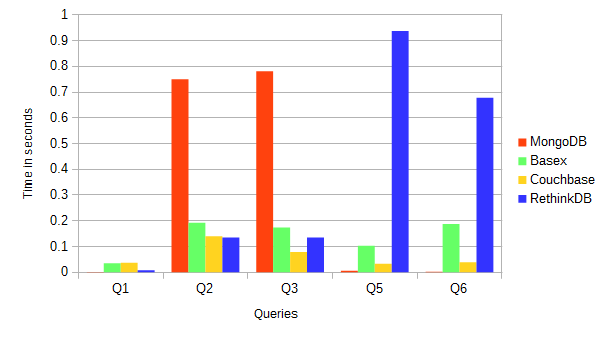
\includegraphics[width=0.44\textwidth]{img/result/1-6}
			%\caption{R-tree structure}
			\label{fig:queries-1-7}
		}
		\centering
		\subfloat[Join Queries (No. 8 to 12)]{
			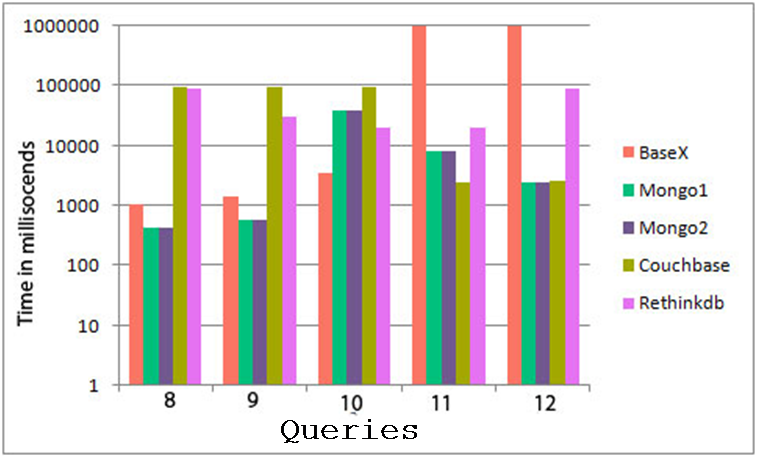
\includegraphics[width=0.44\textwidth]{img/result/8-12}
			%\caption{R-tree}
			\label{fig:queries-8-13}
		}
		
		\centering
		\subfloat[Queries 13 to 20]{
			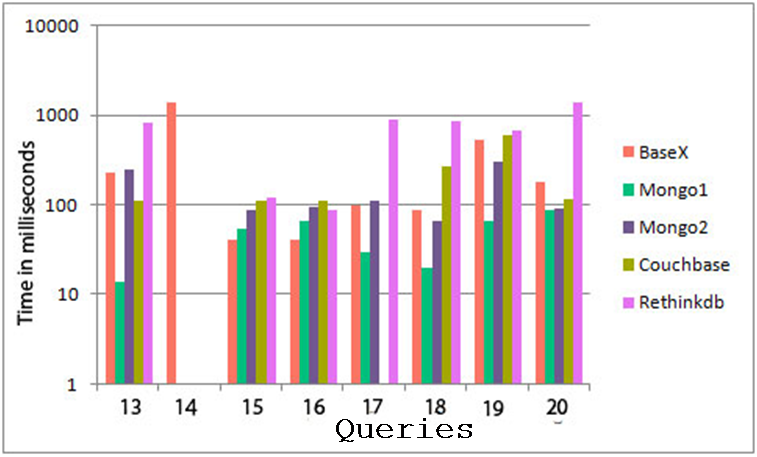
\includegraphics[width=0.44\textwidth]{img/result/13-20}
			%\caption{R-tree}
			\label{fig:queries-13-20}
		}
		\caption{XMark Queries time in XML and NoSQL databases(Mongo1: Mongodb shell, mongo2:through application)}
		\label{fig:query-result}
		
	\end{figure}
		\subsection{Summary}
	\section{Discussion}
	
	\section{Conclusion}\label{conc}
	

	
	\section{Future Work}\label{s.future}
	\begin{appendices}
		\chapter{XMARK Queries}
		\section{MongoDB}
			\label{xmark-queries-mongodb}
\begin{enumerate}[label=Q\arabic*.]
	\item %1
	\begin{lstlisting}[language=JSON,   basicstyle=\scriptsize]
		db.people.find({_id:"person0"},{_id:0,"name":1});
	\end{lstlisting}
	
	\item %2
	\begin{lstlisting}[language=JSON,  basicstyle=\scriptsize]
	db.open_auctions.aggregate([
		{$project:{_id:1,bidder:"$bidder"}},
		{ $unwind: "$bidder"},
		{$group:{_id:"$_id",increase:{$first:"$bidder.increase"}}},
		{$sort:{_id:1}},
		{ $unwind: "$increase"},
		{$project:{_id:0,increase:1}}
	])
	\end{lstlisting}
	
    \item %3
	\begin{lstlisting}[language=JSON,   basicstyle=\scriptsize]
	   db.open_auctions.aggregate([
		{ $unwind: "$bidder"},
		{$group:{_id:"$_id",first:{$first:"$bidder.increase"},last:{$last:"$bidder.increase"}}},
		{$unwind:"$first"},
		{$unwind:"$last"},
		{$project:{_id:1,first:1,last:1,diff:{$gte:["$last",{$multiply:["$first",2]}]}}},
		{$match:{diff:true}},
		{$sort:{_id:1}},
		{$project:{_id:0,increase:{first:"$first",last:"$last"}}}
	   ])
	\end{lstlisting}
	
	
    \item %4
	\begin{lstlisting}[language=JSON,   basicstyle=\scriptsize]
	   []
	\end{lstlisting}
	
	
    \item %5
	\begin{lstlisting}[language=JSON,   basicstyle=\scriptsize]
	   db.closed_auctions.find({price:{$gte:40}}).count()
	\end{lstlisting}
	
    \item %6
	\begin{lstlisting}[language=JSON,   basicstyle=\scriptsize]
	   db.regions.find().count()
	\end{lstlisting}
	
	
    \item %7
	\begin{lstlisting}[language=JSON,   basicstyle=\scriptsize]
	   []
	\end{lstlisting}
	
	
    \item %8
	\begin{lstlisting}[language=JSON,   basicstyle=\scriptsize]
	   function q8() {
        	var ids = new Array();
        	var name = new Array();
        	var closed = new Array();
        	var i=0;
        	db.people.find({},{name:1}).forEach(function(people){
        		ids[i] = people._id;
        		name[ids[i]] = people.name;
        		//closed[ids[i]] = {name:people.name,count:0};
        		i++;
        	});
        	var closed_auc = db.closed_auctions.aggregate([
        		{$project:{_id:1,person:"$buyer.person"}},
        		//{$match:{person:{$in:["person12124","person12883"]}}},
        		{$match:{person:{$in:ids}}},
        		{$group:{_id:"$person",count:{$sum:1}}},
        		{$sort:{count:-1}},
        		{$project:{person:"$_id",count:1,_id:0}}
        	]);
        	if(closed_auc) {
        		var i=0
        		while(closed_auc.hasNext()){
        			var auc = closed_auc.next();
        			var id = auc.person;
        			closed[i] = {"name":name[id],"count":auc.count}
        			name[id] = 0;
        			i++;
        			//printjson(name.indexOf(id));
        		}
        		
        	}/**/
        	var len = closed.length ;
        	var j = 0;
        	for(var i=0; i < ids.length; i++) {
        		if(name[ids[i]] !== 0) {
        		//printjson(i);
        		closed[len+j]	= {"name":name[ids[i]],"count":0};
        		j++;
        		}
        	}
        	//printjson("Execution Time" + end-start);
        	return closed;
        	
        }
	\end{lstlisting}
	
	
    \item %9
	\begin{lstlisting}[language=JSON,   basicstyle=\scriptsize]
	   
	\end{lstlisting}
	
	
    \item %10
	\begin{lstlisting}[language=JSON,   basicstyle=\scriptsize]
	//helper function for Q10.
    var getProfileByCategory = function(catId){
    		var prof = new Array();
    		var i = 0;
    		db.people.find(
    		{"profile.interest":{$exists:true},"profile.interest":{"$elemMatch": {category:catId}}},
    		{name:1, profile:1,address:1}
    		).forEach(function(p){
    			if(!p.address) {
    				p.address = {};
    			}
    			var c = function (value){return ((value) && (typeof value !== "undefined")) ? value : "";}; 
    			prof[i] = {
                          personne: {
                            statistiques: {
                              sexe: c(p.profile.gender),
                              age: c(p.profile.gender),
                              education: c(p.profile.education),
                              revenu: c(p.profile.income)
                            },
                            coordonnees: {
                              nom: p.name,
                              rue: (c(p.address)&&c(p.address.street)),
                              ville: c(p.address.city),
                              pays: c(p.address.country),
                              reseau: {
                                courrier: c(p.emailaddress),
                                pagePerso: c(p.homepage)
                              }
                            },
                            cartePaiement: c(p.creditcard)
                          }
                        }
                            			
    			})
    		return prof;
    		};
    		
    		
	   function q10() {
        	var debugId = "person3"
        	var ids = new Array();
        	var i = 0;
        	var allcategories = new Array();
        	db.people.aggregate([
        	{$match:{"profile.interest":{$exists:true}}},
        	{$project:{_id:1, interest:"$profile.interest"}},
        	{$unwind:"$interest"},
        	{$group:{_id:"$interest.category"}},
        	{$project:{_id:0, category:"$_id"}}
        	]).forEach(function(people){
        		var catId = people.category;
        		ids[i] = {categorie:{id:catId,profile:getProfileByCategory(catId)}}
        		i++;
        	});
        	return ids;
        }
	\end{lstlisting}
	
	
    \item %11
	\begin{lstlisting}[language=JSON,   basicstyle=\scriptsize]
	  function q11() {
    	var start = new Date().getTime();
    	var debugId = "person3"
    	var ids = new Array();
    	var open_auc = function(initial){
    		return db.open_auctions.find({initial:{$lt:initial}},{_id:1}).count();
    	}
    	
    	var i=0;
    	db.people.find({},{_id:1, name:1,"profile.income":1}).forEach(function(people){
    		var income = ((people.profile) && people.profile.income)? people.profile.income/5000:0;
    		ids[i] = {item:{name: people.name,id:people._id,count:open_auc(income)}};
    		i++;
    	});
    	return ids;
        }
	\end{lstlisting}
	
	
    \item %12
	\begin{lstlisting}[language=JSON,   basicstyle=\scriptsize]
	   function q12() {
    	var debugId = "person3"
    	var ids = new Array();
    	var open_auc = function(initial){
    		return db.open_auctions.find({initial:{$lt:initial}},{_id:1}).count();
    	}
    	var i=0;
    	db.people.find({"profile.income":{$exists:true}, "profile.income":{$gt:50000}},{_id:1, name:1,"profile.income":1}).forEach(function(people){
    		var income = ((people.profile) && people.profile.income)? people.profile.income/5000:0;
    		ids[i] = {item:{name: people.name,id:people._id,count:open_auc(income)}};
    		i++;
    	});
    	return ids;

    }
	\end{lstlisting}
	
	\item %13
	\begin{lstlisting}[language=JSON,   basicstyle=\scriptsize]
	    db.regions.find(
		{regions:"australia"},
		{_id:0,name:1,description:1}
        )
	\end{lstlisting}
	
    \item %14
	\begin{lstlisting}[language=JSON,   basicstyle=\scriptsize]
	  db.regions.aggregate([
		{$match:{$text:{$search:"gold"}}},
		{$group:{_id:"$_id"}},
		{$group:{_id:null,count:{$sum:1}}},
		{$project:{_id:0,count:1}}
	])
	\end{lstlisting}
	
    \item %15
	\begin{lstlisting}[language=JSON,   basicstyle=\scriptsize]
	 db.closed_auctions.aggregate([
		{$project:{_id:1,parlist:"$annotation.description.parlist"}},
		{ $unwind: "$parlist"},
		{ $unwind: "$parlist.listitem.parlist"},
		{$project:{_id:1,text:"$parlist.listitem.parlist.listitem.text"}},
		{$match:{$or:[{"text.emph.keyword":{$exists:true}},{"text.emph.keyword.childtext":{$exists:true}},{"text.emph.keyword.child":{$exists:true}}]}},
		{$project:{_id:0,text:"$text.emph.keyword"}}
	])
	\end{lstlisting}
	
    \item %16
	\begin{lstlisting}[language=JSON,   basicstyle=\scriptsize]
	  db.closed_auctions.aggregate([
		{$project:{_id:1,parlist:"$annotation.description.parlist",person:"$seller.person"}},
		{ $unwind: "$parlist"},
		{ $unwind: "$parlist.listitem.parlist"},
		{$project:{_id:1,text:"$parlist.listitem.parlist.listitem.text",person:1}},
		{$match:{"text.emph.keyword":{$exists:true}}},
		{$project:{_id:0,"person.id":"$person"}}
	])
	\end{lstlisting}	

    \item %17
	\begin{lstlisting}[language=JSON,   basicstyle=\scriptsize]
	  db.people.find({homepage:{$exists:false}},{_id:0,person:"$name"})
	])
	\end{lstlisting}	

    \item %18
	\begin{lstlisting}[language=JSON,   basicstyle=\scriptsize]
	  db.open_auctions.aggregate([{$match:{reserve:{$exists:true}}},
		{$project:{_id:0,reserve:{$multiply:["$reserve",2.20371]}}}])
	\end{lstlisting}	

    \item %19
	\begin{lstlisting}[language=JSON,   basicstyle=\scriptsize]
	  db.regions.aggregate([{$sort:{location:1}},
		{$project:{_id:0,"item.name":"$name","item.location":"$location"}}])
	\end{lstlisting}	
    
    \item %20
	\begin{lstlisting}[language=JSON,   basicstyle=\scriptsize]
	  db.people.aggregate([
		{$project:{_id:1,p:"$profile.income"}},
		{$project:{_id:1,con:
			{$cond:[
			  {$gt:["$p",100000]},"preferred",
			  {$cond:[{ $and: [{$lt:["$p", 100000] }, {$gte:["$p", 30000] }] },"standard",
		{$cond:[{$and:[{$lt:["$p",30000]},{$gt:["$p",0]}]},"challange","na"]}
		]}
		]}
		}},
		{$group:{_id:"$con",sum:{$sum:1}}},
		{$project:{_id:1,sum:1}}])
	\end{lstlisting}
\end{enumerate}
\noindent\makebox[\linewidth]{\rule{\paperwidth}{0.4pt}}
\begin{lstlisting}[language=JSON,   basicstyle=\scriptsize, label=mongodb-xmark-index, caption=Secondary indexes in MongoDB's XMark data]
	  db.open_auctions.ensureIndex({
		initial:1
	})
	db.open_auctions.ensureIndex({
		bidder:1
	})
	db.open_auctions.ensureIndex({
		"bidder.increase":1
	})
	
	db.regions.ensureIndex({
		name:1,
		location:1
	})
	db.regions.ensureIndex({
		regions:1
	})
	db.regions.ensureIndex({
		location:1
	})
	db.regions.ensureIndex([
                   { "$**": "text" },
                   { name: "TextIndex" }
                         ])
	db.people.ensureIndex({
		"people.interest":1
	})

	db.closed_auctions.ensureIndex({
		"buyer.person":1
	});
	db.closed_auctions.ensureIndex({price:1})
	\end{lstlisting}

				%\label{xmark-queries}
	\begin{enumerate}[label=Q\arabic*.]
		\paragraph{exact Match}
		\item %1
			Return the name of the person with ID "person0". 
		\begin{lstlisting}[style=XQuery]
			let $auction := doc("xmark.xml") return
				for $b in $auction/site/people/person[@id = "person0"]
			return $b/name/text()
		\end{lstlisting}
		\item %2
			Return the initial increases of all open auctions.
		\begin{lstlisting}[style=XQuery]
			let $auction := doc("xmark.xml") return
    			for $b in $auction/site/open_auctions/open_auction
    			return
                <increase>{ $b/bidder[1]/increase/text() }</increase>
		\end{lstlisting}
		\item %3
			Return the IDs of all open auctions whose current increase is at least twice as high as the initial increase. 
			\begin{lstlisting}[style=XQuery]
				let $auction := doc("xmark.xml") return
					for $b in $auction/site/open_auctions/open_auction
					where zero-or-one($b/bidder[1]/increase/text()) * 2 <=
					$b/bidder[last()]/increase/text()
				return <increase first="{$b/bidder[1]/increase/text()}"
				last="{$b/bidder[last()]/increase/text()}"/>
			\end{lstlisting}	
		
		\item %4
			List the reserves of those open auctions where a certain person issued a bid before another person.
			\begin{lstlisting}[style=XQuery]
			let $auction := doc("xmark.xml") return
			for $b in $auction/site/open_auctions/open_auction
			where some $pr1 in $b/bidder/personref[@person = "person20"],
			$pr2 in $b/bidder/personref[@person = "person51"]
			satisfies $pr1 << $pr2
			return <history>{$b/reserve/text()}</history>
			\end{lstlisting}	
		
		\item %5
			How many sold items cost more than 40?		
		\begin{lstlisting}[style=XQuery]
			let $auction := doc("xmark.xml") return
			count(for $i in $auction/site/closed_auctions/closed_auction
			where $i/price/text() >= 40
			return $i/price)
		\end{lstlisting}	
		\item %6
			How many items are listed on all continents?
		\begin{fakeXML}
			let $auction := doc("xmark.xml") return
			for $b in $auction//site/regions
			return count($b//item)
		\end{fakeXML}	
		\item %7
			How many pieces of prose are in our database?
		\begin{fakeXML}
			let $auction := doc("xmark.xml") return
			for $p in $auction/site
			return count($p//description) + count($p//annotation) + count($p//emailaddress)
		\end{fakeXML}	
		\item %8
			List the names of persons and the number of items they bought.
			
		\begin{fakeXML}
			let $auction := doc("auction.xml") return
				for $p in $auction/site/people/person
				let $a :=
				for $t in $auction/site/closed_auctions/closed_auction
				where $t/buyer/@person = $p/@id
				return $t
			return <item person="{$p/name/text()}">{count($a)}</item>
		\end{fakeXML}	
		\item %9
			List the names of persons and the names of the items they bought in Europe.
		\begin{fakeXML}
			let $auction := doc("xmark.xml") return
			let $ca := $auction/site/closed_auctions/closed_auction return
			let $ei := $auction/site/regions/europe/item
			for $p in $auction/site/people/person
			let $a := for $t in $ca
			where $p/@id = $t/buyer/@person
			return let $n := for $t2 in $ei
			where $t/itemref/@item = $t2/@id
			return $t2
			return <item>{ $n/name/text() }</item>
			return <person name="{ $p/name/text() }">{ $a }</person>
		\end{fakeXML}	
		\item %10
			List all persons according to their interest; use French markup in the result.
		\begin{lstlisting}[style=XQuery,float=ht]
			let $auction := doc($doc)
              for $i in distinct-values($auction/site/people/person/profile/interest/@category)
              let $p :=
                for $t in $auction/site/people/person
                where $t/profile/interest/@category = $i
                return <personne>
              <statistiques>
                <sexe> { $t/profile/gender/text() } </sexe>
                <age> { $t/profile/age/text() } </age>
                <education> { $t/profile/education/text() } </education>
                <revenu> { fn:data($t/profile/@income) } </revenu>
              </statistiques>
              <coordonnees>
                <nom> { $t/name/text() } </nom>
                <rue> { $t/address/street/text() } </rue>
                <ville> { $t/address/city/text() } </ville>
                <pays> { $t/address/country/text() } </pays>
                <reseau>
                  <courrier> { $t/emailaddress/text() } </courrier>
                  <pagePerso> { $t/homepage/text() } </pagePerso>
                </reseau>
              </coordonnees>
              <cartePaiement> { $t/creditcard/text() } </cartePaiement>
            </personne>
              return <categorie>
              <id> { $i } </id>
              { $p }
            </categorie>
		\end{lstlisting}	
		\item  %11
			For each person, list the number of items currently on sale whose price does not exceed 0.02\% of the person’s income.
		\begin{fakeXML}
			let $auction := doc("auction.xml") return
				for $p in $auction/site/people/person
				let $l :=
				for $i in $auction/site/open_auctions/open_auction/initial
				where $p/profile/@income > 5000 * exactly-one($i/text())
				return $i
			return <items name="{$p/name/text()}">{count($l)}</items>
		\end{fakeXML}	
		\item %12
		For each richer-than-average person, list the number of items currently on sale whose price does not exceed 0.02\% of the person’s income.
		
		\begin{fakeXML}
			let $auction := doc("auction.xml") return
			for $p in $auction/site/people/person
			let $l :=
			for $i in $auction/site/open_auctions/open_auction/initial
			where $p/profile/@income > 5000 * exactly-one($i/text())
			return $i
			where $p/profile/@income > 50000
			return <items person="{$p/profile/@income}">{count($l)}</items>
		\end{fakeXML}	
		\item %13
			List the names of items registered in Australia along with their descriptions.
		\begin{fakeXML}
			let $auction := doc("xmark.xml") return
			for $i in $auction/site/regions/australia/item
			return <item name="{ $i/name/text() }">{ $i/description }</item>
		\end{fakeXML}	
		\item %14
			Return the names of all items whose description contains the word ‘gold’.
		\begin{fakeXML}
			let $auction := doc("xmark.xml") return
			for $i in $auction/site//item
			where contains(string(exactly-one($i/description)), "gold")
			return $i/name/text()
		\end{fakeXML}	
		\item %15
			Print the keywords in emphasis in annotations of closed auctions.
		\begin{fakeXML}
			let $auction := doc("xmark.xml") return
			for $a in $auction/site/closed_auctions/closed_auction/annotation/description/
			parlist/listitem/parlist/listitem/text/emph/keyword/text()
			return <text>{ $a }</text
		\end{fakeXML}	
		\item %16
			Return the IDs of those auctions that have one or more keywords in emphasis.
		\begin{fakeXML}
			let $auction := doc("xmark.xml") return
			for $a in $auction/site/closed_auctions/closed_auction
			where not(empty($a/annotation/description/parlist/listitem/parlist/listitem/text/
			emph/keyword/text()))
			return <person id="{ $a/seller/@person }"/>
		\end{fakeXML}	
		\item %17	
			Which persons don’t have a homepage?
		\begin{fakeXML}
			let $auction := doc("xmark.xml") return
			for $p in $auction/site/people/person
			where empty($p/homepage/text())
			return <person name="{ $p/name/text() }"/>
		\end{fakeXML}	
		\item %18
			Convert the currency of the reserve of all open auctions to another currency.
		\begin{fakeXML}
			declare namespace local = "http://www.foobar.org";
			declare function local:convert($v as xs:decimal?) as xs:decimal? {
				2.20371 * $v (: convert Dfl to Euro :)
			};
			let $auction := doc("xmark.xml") return
			for $i in $auction/site/open_auctions/open_auction
			return local:convert(zero-or-one($i/reserve))
		\end{fakeXML}	
		\item %19
			Give an alphabetically ordered list of all items along with their location.
		\begin{fakeXML}
			let $auction := doc("xmark.xml") return
			for $b in $auction/site/regions//item
			let $k := $b/name/text()
			order by zero-or-one($b/location) ascending empty greatest
			return <item name="{ $k }">{ $b/location/text() }</item>
		\end{fakeXML}	
		\item %20
			Group customers by their income and output the cardinality of each group.
		\begin{fakeXML}
			let $auction := doc("xmark.xml") return
			<result>
			<preferred>{
				count($auction/site/people/person/profile[@income >= 100000])
			}</preferred>
			<standard>{
				count($auction/site/people/person/
				profile[@income < 100000 and @income >= 30000])
			}</standard>
			<challenge>{
				count($auction/site/people/person/profile[@income < 30000])
			}</challenge>
			<na>{
				count(for $p in $auction/site/people/person
				where empty($p/profile/@income)
				return $p)
			}</na>
			</result>
		\end{fakeXML}
			
		
	\end{enumerate}
	\end{appendices}

	\bibliographystyle{plainnat}
	\bibliography{ref}
	\newpage
	\listoffigures
	\newpage
	\listoftables
	\newpage
	\lstlistoflistings
	%%%%%%%%%%%%%%%%%%%%%abbreviate
	\abbrev{XML}{Extensible Markup Language}
	\abbrev{JSON}{JavaScript Object Notation}
	\abbrev{VM}{Virtual Machine}
	\abbrev{JVM}{Java Virtual Machine}
	\abbrev{IPC}{Inter-process Communication}
	\abbrev{SDK}{Software Development Kit}
	\abbrev{GUI}{Graphical User Interface}
	\abbrev{XML}{Extensible Markup Language}
	\abbrev{HTML}{Hypertext Markup Language}
	\abbrev{DOM}{Document Object Model}
	\abbrev{IR}{Information Retrieval}
	\abbrev{CB}{Couchbase Server}	
	\abbrev{SDK}{Software Development Kit}
	\abbrev{CAS}{Check-and-Set}
	\abbrev{SDK}{ Software Development Kit}
	
	
\end{document}	
